\begin{center}
\textbf{第十二届“中关村青联杯”全国研究生数学建模竞赛}
\end{center}

\begin{tabular}{l l}
学校 & 空军预警学院 \\
\hline
参赛队号 & 90047006 \\
\hline
队员姓名 & \begin{tabular}{l l}
1. & 熊智敏 \\
2. & 王庚 \\
3. & 漆家辉
\end{tabular}
\end{tabular}

\begin{flushright}
参赛密码 \underline{\hspace{2cm}} \\
(由组委会填写)
\end{flushright}

\begin{center}
\textbf{参赛密码} \underline{\hspace{3cm}} \\
(由组委会填写)
\end{center}

\begin{center}
\includegraphics[width=0.2\textwidth]{image1.png} \quad
\includegraphics[width=0.2\textwidth]{image2.png} \quad
\includegraphics[width=0.3\textwidth]{image3.png} \quad
\includegraphics[width=0.2\textwidth]{image4.png}
\end{center}

\begin{center}
\textbf{第十二届“中关村青联杯”全国研究生} \\
\textbf{数学建模竞赛}
\end{center}

\begin{center}
\textbf{题目} \underline{E. 数控加工刀具运动的优化控制}
\end{center}

\begin{center}
\textbf{摘 要:}
\end{center}

针对数控加工刀具运动的优化控制问题,在充分研究 $S$ 型加减速度算法特点的基础上,提出针对折线型优化控制的前瞻法改进 $S$ 型加减速度算法和针对圆弧线型优化控制的改进型三角函数加减速度算法,建立了相应的控制算法模型,利用实例进行验证,得到了较好的效果,体现了模型的合理性,具有一定的指导意义和实用价值。

针对问题一,主要研究了折线交点的速度变化的问题,利用前瞻算法计算出折线交点的最大允许速度,建立了基于前瞻法 $S$ 型加减速改进算法模型,分析了初始速度 $v_{s}$ 和末速度 $v_{e}$ 对模型的影响。利用所建模型,在假设插补周期 $T=1\text{ms}$ 的前提下,求解得到 $90^\circ$ 和 $135^\circ$ 的最大转角速度分别为 $4.24\text{mm}/\text{s}$ 和 $7.84\text{mm}/\text{s}$。最后在误差允许范围内,改变加工路径,增大了交点的最大允许速度,利用所建模型,求解得到 $90^\circ$ 和 $135^\circ$ 的最大转角速度分别为 $11.59\text{mm}/\text{s}$ 和 $15.38\text{mm}/\text{s}$。

针对问题二,首先在考虑弦高误差的限制下,给出圆弧粗插补方案,进而在考虑分辨率的情况下,给出了插补点的实时搜索算法;其次,分情况对直线与圆弧之间的转接进行分析,得到实时加工算法;然后,利用该算法对实例进行求解,得到加工方案,其加工时间 $103.3890\text{s}$,最大误差 $0.9976\mu\text{m}$;最后,从理论和仿

\begin{center}
- 1 -
\end{center}

\section*{真分别分析了圆弧半径对加工效率的影响,得到结论:半径越大,加工效率越高。}

针对问题三,在考虑瞬时启动速度及加速度的情况下,对 $S$ 型曲线加减速算法的参数进行修正,并对实例进行求解和对比分析,观察发现在短距离加工时,速度变化剧烈,不能平滑地过渡折线交点;并且不考虑瞬时启动速度及加速度的情况下,进行仿真实验比较,实际仿真结果显示考虑瞬时启动速度及加速度的情况下,机床运行时间更短,算法效率更高。

针对问题四,在前三问的基础上,充分分析 $S$ 型算法的优缺点。提出基于改进型三角函数算法,建立了改进型三角函数的加减速控制模型。其中,改进型三角函数改进了三角函数算法不能满足以最大速度 $v_{\text{max}}$ 匀速加工,在仿真实验中并且利用加加速度 $J$ 按照三角函数线型曲线变化,在相较于 $S$ 型加减速算法的运行时间差别不大的情况下,可以使得速度和加速度都满足平滑性变化,改善了加工过程的稳定性,提高了机床加工的精度,减小了对刀具的损耗。

\section*{关键词:S 型曲线加减速 数控加工 前瞻算法 插补模型 路径优化 改进型三角函数算法}

\section*{目录}
\begin{itemize}
    \item 一、问题的重述 \dotfill 5
    \begin{itemize}
        \item 1.1 问题由来 \dotfill 5
        \item 1.2 问题要求 \dotfill 5
        \item 1.3 问题的提出 \dotfill 5
    \end{itemize}
    \item 二、问题的假设 \dotfill 5
    \item 三、符号说明 \dotfill 6
    \item 四、问题一的分析与求解 \dotfill 6
    \begin{itemize}
        \item 4.1 问题一的分析 \dotfill 6
        \item 4.2 相邻折线型线连接点处夹角与进给速度的关系 \dotfill 8
        \item 4.3 刀具在折线上运动的控制模型 \dotfill 9
        \begin{itemize}
            \item 4.3.1 理想型 S 型加减速度算法 \dotfill 9
            \item 4.3.2 非理想 S 型加减速度算法 \dotfill 11
            \item 4.3.3 基于前瞻法改进 S 型加减速度算法 \dotfill 12
            \item 4.3.4 基于前瞻法改进 S 型加减速度算法控制流程 \dotfill 18
        \end{itemize}
        \item 4.4 模型应用 \dotfill 19
        \begin{itemize}
            \item 4.4.1 刀具运动状态模型 \dotfill 19
            \item 4.4.2 折线交点角度与速度模型 \dotfill 20
            \item 4.4.3 刀具在折线上运动速度控制模型 \dotfill 20
        \end{itemize}
        \item 4.5 问题一的求解 \dotfill 21
        \item 4.6 问题一的进一步求解 \dotfill 24
    \end{itemize}
    \item 五、问题二的分析与求解 \dotfill 25
    \begin{itemize}
        \item 5.1 问题二的分析 \dotfill 25
        \begin{itemize}
            \item 5.1.1 弦高误差分析 \dotfill 25
            \item 5.1.2 圆弧轨迹插补方案 \dotfill 26
            \item 5.1.3 搜索算法 \dotfill 27
        \end{itemize}
        \item 5.2 直线和圆弧转接分析 \dotfill 28
        \begin{itemize}
            \item 5.2.1 直线与圆弧相切分析 \dotfill 28
            \item 5.2.2 直线与圆弧不相切分析 \dotfill 29
        \end{itemize}
    \end{itemize}
\end{itemize}

\begin{itemize}
    \item 5.3 问题二的模型求解 \dotfill -30-
    \item 5.3.1 算法控制流程 \dotfill -30-
    \item 5.3.2 算例结果 \dotfill -31-
    \item 5.4 圆弧半径的变化对算法效率的影响 \dotfill -33-
    \item 六、问题三的分析与求解 \dotfill -34-
    \item 6.1 问题三的分析 \dotfill -34-
    \item 6.1.1 瞬时速度的影响的因素 \dotfill -34-
    \item 6.1.2 瞬时加速度的影响的因素 \dotfill -35-
    \item 6.2 问题三的模型建立 \dotfill -35-
    \item 6.2.1 考虑瞬时量的理想S型算法 \dotfill -35-
    \item 6.2.2 考虑瞬时量的前瞻S型算法 \dotfill -37-
    \item 6.3 问题三的模型求解 \dotfill -38-
    \item 七、问题四的分析与求解 \dotfill -41-
    \item 7.1 问题四的分析 \dotfill -41-
    \item 7.2 S型加减速控制算法的优缺点 \dotfill -41-
    \item 7.3 三角函数加减速算法 \dotfill -42-
    \item 7.4 四次位移加减速控制算法 \dotfill -45-
    \item 7.5 三种加减速控制方法的比较 \dotfill -46-
    \item 八、模型总结及其改进 \dotfill -49-
    \item 参考文献: \dotfill -49-
    \item 附录: \dotfill -50-
\end{itemize}

\section*{一、问题的重述}

\subsection{1.1 问题由来}

机械制造技术的指标最关键的三个方面是速度、精度和效率。而数控加工技术中一个重要的环节便是由数控系统对输入的指令进行信息处理和设计刀具的运动轨迹。刀具的实际运动轨迹的平滑流畅,速度稳定与否会直接影响到后期零件加工的质量和成本,所以刀具轨迹运动的优化一直是数控加工研究的一个热点。

\subsection{1.2 问题要求}

在数控机床所提供的精度、速度、加速度等限制条件下,数控加工刀具运动的优化控制就是寻求合理方法控制机床刀在各坐标轴方向上的运动,通过对其运动轨迹的优化进而提高其加工效率,并且实现高速有效柔性加减控制。除了较为直观的直线切割,对于一般曲线的加工,在满足误差要求的条件下,数控加工控制过程就是通过利用插补算法等方式,将曲线切割转换为若干小直线段的组成完成加工刀具的运动轨迹,同时计算出刀具运动对应的速度、加速度、轨迹等参数。

\subsection{1.3 问题的提出}

1、完成相邻两折线段夹角为 $90^\circ$ 和 $135^\circ$ 时的刀具加工路线并讨论通过折线交点时对应各坐标运动速度的变化;

2、完成加工型线是由直线段和圆弧段(相切或不相切)组成的连续曲线的刀具加工路线并讨论通过折线交点时对应各坐标运动速度的变化;建立实时加工优化控制算法,讨论圆弧半径的变化对算法效率的影响;并应用所建立的模型对下面的加工路径示例进行检验;

3、在第 2 问基础上,考虑瞬时启动加速度及瞬时启动速度,建立相对应的实时加工优化控制算法;并应用所建立的模型对下面的加工路径示例进行检验;

4、结合前 3 问,分析 S 型曲线的加减速控制方法的优缺点,在满足精度和速度要求的条件下,建立能提高机床运行平稳性的优化控制运动模型(如刀具在各坐标轴方向上的运动满足加加速度连续变化等)。

\section*{二、问题的假设}

1. 刀具具体形状假想为一个质点。

2. 刀具实际路径由一系列直线段组成。

3. 在折线交点处允许的最大进给速度方向为下一段直线段指向方向可以突变。

4. 假设机床刀具运动的插补周期一定,此处选择 $T = 1ms$。

5. 在 S 型曲线加减速过程中,为了更快加速或减速,机床的加加速度为限定为零或最大值。

6. 不考虑数控系统的操作指令传递和操作造成的时延问题。

\section*{三、符号说明}

\begin{itemize}
    \item $T$: 插补周期。
    \item $J_{const}$: 加加速度最大值。
    \item $\nu_{\max}$: 最大限制进给速度。
    \item $a_{\max}$: 最大限制加速度。
    \item $\delta_{h}$: 最大插补弦高误差。
    \item $ds$: 分辨率。
    \item $\nu_{s}$: 初始速度。
    \item $\nu_{e}$: 末尾速度。
    \item $L$: 给定路径长度。
    \item $S_{d}$: 减速区路径长度。
    \item $S_{a}$: 加速区路径长度。
    \item $t_{\mathrm{m}}$: 理想情况下$T_{1}$时间长度。
    \item $\alpha$: 两折线间夹角。
    \item $\nu_{0}$: 瞬时速度。
    \item $a_{0}$: 瞬时加速度。
    \item $t_{am}$: 表示的整个加速运行时间
    \item $a_{ramax}$: 表示实际采用的最大加速度
    \item $j_{\max}$: 表示最大的加加速度值
    \item $T_{i}(i=1,2,\cdots,7)$: $S$型加减速度算法各阶段对应时间。
\end{itemize}

\section*{四、问题一的分析与求解}

\subsection{问题一的分析}

正常数控操作中,待加工型可能比较复杂,因此有三轴,六轴和八轴控制系

\begin{figure}[h]
    \centering
    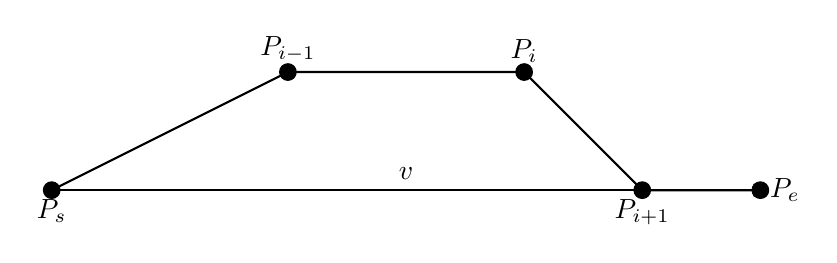
\begin{tikzpicture}[scale=1.5]
        \draw[->, thick] (0,0) -- (6,0) node[midway, above] {$v$};
        
        \filldraw (0,0) circle (2pt) node[anchor=north] {$P_s$};
        \filldraw (2,1) circle (2pt) node[anchor=south] {$P_{i-1}$};
        \filldraw (4,1) circle (2pt) node[anchor=south] {$P_i$};
        \filldraw (5,0) circle (2pt) node[anchor=north] {$P_{i+1}$};
        \filldraw (6,0) circle (2pt) node[anchor=west] {$P_e$};
        
        \draw[thick] (0,0) -- (2,1) -- (4,1) -- (5,0) -- (6,0);
    \end{tikzpicture}
    \caption{刀具折线运动轨路线迹}
    \label{fig:tool_path}
\end{figure}

而对单一路径直线如 $P_{i-1}P_i$ 上进行加工,其易于实现,精度也较高,但若是折线型路径 $P_sP_e$,则需要考虑转折点的情况。也就是说刀具折线运动轨迹是折线间的夹角以及夹角两侧折线共同组成的。为了实现折线路径上刀具速度控制优化,可以将刀具的运动轨迹模型分解为两段折线上的 $S$ 型加减速运动以及折线交点处转角运动。同时分析这个过程中刀具的运动状态的改变以及转角处各坐标的速度变化情况。

如图 \ref{fig:tool_path} 所示,刀具折线运动轨迹中,在 $P_i$ 点附近出现折线转弯,为保证转角处的轨迹精度,避免发生过切或由于速度过大产生的刀具震动问题,在转角处必须限制转角进给速度,即 $P_i$ 点的进给速度必须小于或等于由折线角度确定的最大允许进给速度。

为此,数控优化速度控制系统需根据转角允许最大进给速度的大小以及最大加速度和加加速度变化的约束,在 $P_i$ 点之前的 $P_{i-1}$ 点开始减速,这样便可以使到达 $P_{i+1}$ 点时速度正好满足允许速度的要求,并在可以在经过 $P_{i+1}$ 点后逐步加速,使其进给速度恢复正常。

另一方面,由于问题一是在加工误差恒定的情况下讨论刀具运动,那么还应该给出刀具经过折线点前后,各坐标轴种运动状态的变化情况。为了表示刀具运动过程中,各种运动量的变化情况,首先要建立坐标系,将刀具相对于机床的切割运动转化为坐标系中的点迹运动,完成刀具运动轨迹的建模。由于本题不考虑工件在深度方向上的加工,即运动层面是平面运动,所以只需建立二维直角坐标系 $XOY$,其运动过程中各个运动量的向量关系如下:

\begin{figure}[h]
    \centering
    \includegraphics[width=0.8\textwidth]{image1.png}
    \caption{运动量的坐标表示}
    \label{fig:4.2}
\end{figure}

\subsection{相邻折线型线连接点处夹角与进给速度的关系}

如图 \ref{fig:4.3} 所示,$\alpha$ 是相邻折线之间的夹角,即第一条折线终点处的加工进给方向与第二条折线起点处的加工进给方向的夹角。$B$ 点为相邻两条折线的连接点,规定夹角 $\alpha$ 的范围为 $0^\circ \sim 180^\circ$。那么,当 $\alpha = 0^\circ$ 时,对 $B$ 点处的进给速度大小是没有限制,但当 $\alpha = 180^\circ$ 时,$B$ 点处的进给速度必须为零。可以看出,在 $0^\circ \sim 180^\circ$ 之间,$\alpha$ 越大,所允许的 $B$ 点进给速度值就越小。下面给出推导夹角 $\alpha$ 对 $B$ 点进给速度值的限制影响的公式。

\begin{figure}[h]
    \centering
    \includegraphics[width=0.8\textwidth]{image2.png}
    \caption{相邻折线连接处的进给速度}
    \label{fig:4.3}
\end{figure}

刀具沿折线 $AB$ 加工到折线终点 $B$ 时的进给速度为 $v_e$,接下来应该进入下一个路径段 $BC$ 进行加工,在 $BC$ 段起点处的进给速度 $v_s$ 与 $v_e$ 的夹角为 $\alpha$,大小相同。由此计算在该相邻折线连接处的加速度大小为

\begin{equation}
a = \frac{2v_e \sin \frac{\alpha}{2}}{T}
\tag{4.1}
\end{equation}

上式中 \( T \) 为插补周期。由于数控系统要求有最大加速度的限制,即:

\begin{equation}
a = \frac{2v_e \sin \frac{\alpha}{2}}{T} \leq a_{\text{max}}
\tag{4.2}
\end{equation}

由上式可以得出对相邻折线连接处进给速度大小的限制为:

\begin{equation}
v_e \leq \frac{T a_{\text{max}}}{2 \sin \frac{\alpha}{2}}
\tag{4.3}
\end{equation}

问题中已知数控系统最大限定加速度值为 \( 0.6 \, m/s^2 \),插补周期为 \( 1 \, ms \),则相邻路折线之间夹角 \( 0^\circ \sim 150^\circ \) 与允许进给速度值之间的对应关系如图 4.4 所示。

\begin{figure}[h]
\centering
\includegraphics[width=\textwidth]{image.png}
\caption{不同转折角度下转折点允许的最大可运行速度}
\end{figure}

图 4.4 折线之间夹角与允许进给速度值之间的对应关系

\subsection{4.3 刀具在折线上运动的控制模型}

\subsubsection{4.3.1 理想型 S 型加减速度算法}

假设刀具运动加速度曲线从 0 达到最大值和从最大值到 0 所用的时间相等,此时间定为系统的一个特性时间常数 \( t_m \),其应满足 \( t_m \leq \frac{v_{\text{max}}}{a_{\text{max}}} \),取 \( t_m = \frac{v_{\text{max}}}{2a_{\text{max}}} \),据此假设,其中 \( T_i (i = 1, 2, \cdots, 7) \) 为 S 型加减速度算法各阶段对应时间。

\begin{equation}
T_1 = T_3 = T_5 = T_7 = t_m
\tag{4.4}
\end{equation}

从而:

\begin{equation}
J = J_1 = J_3 = J_5 = J_7 = \frac{a_{\text{max}}}{t_m}
\tag{4.5}
\end{equation}

但是(4.4)的前提条件是:运行过程中最大加速度能达到。若这个条件不成立,则由下式代替
\begin{equation}
\begin{cases}
T_{1}=T_{3} \\
T_{5}=T_{7}
\end{cases}
\tag{4.6}
\end{equation}
由题目中可得 S 型算法的各段运动方程如下:

(1) 加加速段
\begin{equation}
\begin{cases}
J=J_{const} \\
a=Jt \\
V=\frac{1}{2}Jt^{2} \quad t \in (0,T_{1}]
\end{cases}
\tag{4.7}
\end{equation}
其中 $T_{1}=a_{\max } / J_{const}$,这个过程中加速度达到最大 $a_{\max }$,加速度和速度都在增加。

(2) 匀加速段
\begin{equation}
\begin{cases}
J=0 \\
a=a_{\max } \\
V=\frac{1}{2}J_{const}T_{1}^{2}+a_{\max }(t-T_{1}) \quad t \in (T_{1},T_{1}+T_{2}]
\end{cases}
\tag{4.8}
\end{equation}
其中 $T_{2}=(V_{\max }-J_{const}T_{1}^{2}) / a_{\max }$,这个过程中加速度不变,速度在增加。

(3) 减加速段
\begin{equation}
\begin{cases}
J=J_{const} \\
a=a_{\max }-J(t-T_{1}-T_{2}) \\
V=\frac{1}{2}J_{const}T_{1}^{2}+a_{\max }T_{2}+a_{\max }(t-T_{1}-T_{2})-\frac{1}{2}J(t-T_{1}-T_{2})^{2} \quad t \in (T_{1}+T_{2},2T_{1}+T_{2}]
\end{cases}
\tag{4.9}
\end{equation}
这个过程中加速度在减小,速度在增加,一直增加到 $V_{\max }$,当 $t=2T_{1}+T_{2}$ 时,$V=V_{\max }$。

(4) 匀速段
\begin{equation}
\begin{cases}
J=0 \\
a=0 \\
V=V_{\max } \quad t \in (2T_{1}+T_{2},2T_{1}+T_{2}+T_{4}]
\end{cases}
\tag{4.10}
\end{equation}
这个过程中加速度为 0,速度保持 $V_{\max }$ 不变,$T_{3}$ 的长短由路径长度决定。

(5) 加减速段

\begin{equation}
\begin{cases}
J = J_{const} \\
a = -J(t - 2T_1 - T_2 - T_3) \\
V = V_{\text{max}} - \frac{1}{2}J(t - 2T_1 - T_2 - T_4)^2 \quad t \in (2T_1 + T_2 + T_4, 3T_1 + T_2 + T_4]
\end{cases}
\tag{4.11}
\end{equation}

这个过程中加速度在增加,速度在减小,这段其实与减加速段是对称的。

(6) 匀减速段

\begin{equation}
\begin{cases}
J = 0 \\
a = -a_{\text{max}} \\
V = V_{\text{max}} - \frac{1}{2}J_{\text{const}}T_1^2 - a_{\text{max}}(t - 3T_1 - T_2 - T_4) \\
t \in (3T_1 + T_2 + T_4, 3T_1 + 2T_2 + T_4]
\end{cases}
\tag{4.12}
\end{equation}

这个过程中加速度保持 $-a_{\text{max}}$ 不变,速度在减小,这段其实与匀加速段是对称的。

(7) 减减速段

\begin{equation}
\begin{cases}
J = J_{\text{const}} \\
a = -a_{\text{max}} + J(t - 3T_1 - 2T_2 - T_4) \\
V = V_{\text{max}} - \frac{1}{2}JT_1^2 - a_{\text{max}}T_2 - a_{\text{max}}(t - 3T_1 - 2T_2 - T_4) + \frac{1}{2}J(t - 3T_1 - 2T_2 - T_4)^2 \\
t \in (3T_1 + 2T_2 + T_4, 4T_1 + 2T_2 + T_4]
\end{cases}
\tag{4.13}
\end{equation}

这个过程中加速度在减小直到为 0,速度也在减小直到为 0,当 $t = 4T_1 + 2T_2 + T_3$ 时,$V = 0$。这段其实与加速段是对称的。

### 4.3.2 非理想 S 型加减速算法

因为实际加工路径中每段路径长度较短,由公式 $t_{\text{m}} = \frac{v_{\text{max}}}{2a_{\text{max}}}$ 推导出 $t_{\text{m}}$。将 $t_{\text{m}}$ 带入加速阶段,计算出的该段末速度大于 $v_{\text{max}}$。所以此时最大加速度 $a_{\text{max}}$ 不能达到,即不考虑匀加速段和匀减速段。所以建立非理想 S 型算法的各段运动方程如下:

(1) 加加速段

\begin{equation}
\begin{cases}
J = J_{\text{const}} \\
a = Jt \\
V = \frac{1}{2}Jt^2 \quad t \in (0, T_1]
\end{cases}
\tag{4.14}
\end{equation}

加速度和速度都在增加。

(2) 减加速段

\begin{equation}
\begin{cases}
J = J_{const} \\
a = a_{\max} - J(t - T_1 - T_2) \\
V = \frac{1}{2} J_{const} T_1^2 + a_{\max} T_2 + a_{\max}(t - T_1 - T_2) - \frac{1}{2} J(t - T_1 - T_2)^2 \\
\quad t \in (T_1 + T_2, 2T_1 + T_2]
\end{cases}
\tag{4.15}
\end{equation}

这个过程中加速度在减小,速度在增加,一直增加到 \( V_{\max} \),当 \( t = 2T_1 + T_2 \) 时, \( V = V_{\max} \)。

(3) 匀速段

\begin{equation}
\begin{cases}
J = 0 \\
a = 0 \\
V = V_{\max} \quad t \in (2T_1 + T_2, 2T_1 + T_2 + T_3]
\end{cases}
\tag{4.16}
\end{equation}

这个过程中加速度为 0,速度保持 \( V_{\max} \) 不变,\( T_3 \) 的长短由路径长度决定。

(4) 加减速段

\begin{equation}
\begin{cases}
J = J_{const} \\
a = -J(t - 2T_1 - T_2 - T_3) \\
V = V_{\max} - \frac{1}{2} J(t - 2T_1 - T_2 - T_4)^2 \quad t \in (2T_1 + T_2 + T_4, 3T_1 + T_2 + T_4]
\end{cases}
\tag{4.17}
\end{equation}

这个过程中加速度在增加,速度在减小,这段其实与减加速段是对称的。

(5) 减减速段

\begin{equation}
\begin{cases}
J = J_{const} \\
a = -a_{\max} + J(t - 3T_1 - 2T_2 - T_4) \\
V = V_{\max} - \frac{1}{2} J T_1^2 - a_{\max} T_2 - a_{\max}(t - 3T_1 - 2T_2 - T_4) \\
\quad + \frac{1}{2} J(t - 3T_1 - 2T_2 - T_4)^2 \quad t \in (3T_1 + 2T_2 + T_4, 4T_1 + 2T_2 + T_4]
\end{cases}
\tag{4.18}
\end{equation}

这个过程中加速度在减小直到为 0,速度也在减小直到为 0,当 \( t = 4T_1 + 2T_2 + T_3 \) 时,\( V = 0 \)。这段其实与加加速段是对称的。

\subsection*{4.3.3 基于前瞻法改进 S 型加减速度算法}

理想型 S 型加减速度算法可以完成单段折线上刀具的速度控制。在实际使用中,为了实现 \( N \) 段轨迹的速度规划,每次执行一次算法都要进行加减速过程,每一次算法执行完后速度都要降到零,这种方式最大的缺点就是加工效率低下,而且由于运动停顿较多,导致加工表面质量低,而且频繁启动和停止使得机床要频繁启停,对机床的机械系统及电气系统都不利。为了减少此类问题,实际情况中需要对连续折线轨迹上刀具的速度进行控制。这里的连续加工轨迹是指一系列首尾相连的直线、圆弧构成的轨迹。连接方式有:直线接直线、直线接圆弧、圆弧接直线、圆弧接圆弧等。相比于单段折线运动控制,连续加工轨迹需要加入折

线夹角进给速度的计算与判断,这样就能够使每段直线或圆弧的始末速度可能不为零,进而提高刀具加工效率。

基于前瞻处理的改进 $S$ 型加减速度算法将为直线、圆弧构成的一条完整的轨迹作为一个整体规划,这个整体的起点速度和终点速度是零,但在各转接点尽可能不要将速度降为零。由于 $S$ 型加减速度算法在实际运行过程中,不可能完成 $S$ 型算法 7 个阶段完整的运行,所以应根据不同情况分类讨论。由于起始和终止速度的不同,故速度曲线也不同,所以以起始和终止速度分类为讨论基础参数。

基于前瞻处理的改进 $S$ 型加减速度算法模型讨论如下:

(1) $\nu_{s}=\nu_{e}=\nu_{\max }$

这种情况下,只有匀速运行阶段,无需进行加减速处理。

(2) $\nu_{s}=\nu_{\max }$ 且 $0<\nu_{e}<\nu_{\max }$

该阶段没有加速过程,只有减速过程,此时 $T_{1}=T_{2}=T_{3}=0$ 。

① $\nu_{e}<\nu_{\max }-a_{\max } t_{m}$

该阶段最大加速度能够达到,则 $T_{5}=T_{7}=t_{m}, \quad T_{6}=\frac{\nu_{\max }-\nu_{e}}{a_{\max }}-t_{m}, \quad J T_{5}=a_{\max }$ 。

其减速区长度为 $S_{d}=\frac{1}{2}\left(\nu_{\max }+\nu_{e}\right)\left(\frac{\nu_{\max }-\nu_{e}}{a_{\max }}+t_{m}\right)$ 。

在这种情况下,根据 $L$ 与 $S_{d}$ 的大小不同,又可以分为以下三种情况:

a) $L>S_{d}$

运行过程:匀速 $\Rightarrow$ 加减速 $\Rightarrow$ 匀减速 $\Rightarrow$ 减减速。

b) $L=S_{d}$

$T_{4}=0$ ,运行过程:加减速 $\Rightarrow$ 匀减速 $\Rightarrow$ 减减速。

c) $L<S_{d}$

$T_{4}=0$ ,运行过程:加减速 $\Rightarrow$ 匀减速 $\Rightarrow$ 减减速。

② $\nu_{e} \geqslant \nu_{\max }-a_{\max } t_{m}$

该阶段最大加速度不能够达到,则 $T_{6}=0, T_{5}=\sqrt{\frac{\nu_{\max }-\nu_{e}}{J}}, S_{d}=2 \nu_{\max } T_{5}-J T_{5}^{3}$ 。

在这种情况下,根据 $L$ 与 $S_{d}$ 的大小不同,同样可以分为以下三种情况:

a) $L>S_{d}$

运行过程:匀速$\Rightarrow$加减速$\Rightarrow$减减速。

b) $L=S_{d}$

$T_{4}=0$,运行过程:加减速$\Rightarrow$减减速。

c) $L<S_{d}$

$T_{4}=0$,运行过程:加减速$\Rightarrow$减减速。但到达终点时无法达到末速度$v_{e}$。

此时,通过$L=2v_{\max }T_{5}-JT_{5}^{3}$解得$T_{5}$,由$T_{5}=\sqrt{\frac{v_{\max }-v_{e}}{J}}$可知$v_{s}=v_{e}+JT_{5}^{2}$,重新确定各段时间,进而对起始速度进行修正。

(3) $v_{e}=v_{\max }$且$0<v_{s}<v_{\max }$

该阶段没有减速过程只有加速过程。此时$T_{5}=T_{6}=T_{7}=0$。

① $v_{s}<v_{\max }-a_{\max }t_{m}$

该阶段最大加速度能够达到,则$T_{1}=T_{3}=t_{m}$,$T_{2}=\frac{v_{\max }-v_{e}}{a_{\max }}-t_{m}$,$JT_{1}=a_{\max }$。

减速区长度$S_{a}=\frac{1}{2}\left(v_{\max }+v_{s}\right)\left(\frac{v_{\max }-v_{s}}{a_{\max }}+t_{m}\right)$。

在这种情况下,根据$L$与$S_{a}$的大小不同,又可以分为以下三种情况:

a) $L>S_{a}$

运行过程:加加速$\Rightarrow$匀加速$\Rightarrow$减加速$\Rightarrow$匀速。

b) $L=S_{a}$

$T_{4}=0$,运行过程:加加速$\Rightarrow$匀加速$\Rightarrow$减加速。

c) $L<S_{a}$

$T_{4}=0$,运行过程:加加速$\Rightarrow$匀加速$\Rightarrow$减加速。

② $v_{s} \geqslant v_{\max }-a_{\max }t_{m}$

该阶段最大加速度不能够达到,则$T_{2}=0$,$T_{1}=\sqrt{\frac{v_{\max }-v_{s}}{J}}$,$S_{a}=2v_{s}T_{1}-JT_{1}^{3}$。

在这种情况下,根据$L$与$S_{a}$的大小不同,同样可以分为以下三种情况:

a) $L > S_{a}$

运行过程:加加速 $\Rightarrow$ 减加速 $\Rightarrow$ 匀速。

b) $L = S_{a}$

$T_{4} = 0$,运行过程:加加速 $\Rightarrow$ 减加速。

c) $L < S_{a}$

$T_{4} = 0$,运行过程:加加速 $\Rightarrow$ 减加速。

(4) $0 < v_{s} < v_{\text{max}}$ 且 $0 < v_{e} < v_{\text{max}}$

由于 $v_{e}$,$v_{s}$ 大小不同,可分为四种情况讨论。

① $v_{s} < v_{\text{max}} - a_{\text{max}} t_{m}$ 且 $v_{e} < v_{\text{max}} - a_{\text{max}} t_{m}$

最大加速度能够达到,则 $JT_{1} = JT_{5} = a_{\text{max}}$,取 $T_{1} = T_{3} = t_{m}$,$T_{2} = \frac{v_{\text{max}} - v_{e}}{a_{\text{max}}} - t_{m}$,$T_{5} = T_{7} = t_{m}$,$T_{6} = \frac{v_{\text{max}} - v_{e}}{a_{\text{max}}} - t_{m}$。由 $T_{4} \geq 0$ 可得

\[
L \geq \frac{v_{\text{max}}^{2}}{a_{\text{max}}} - \frac{1}{2a_{\text{max}}} \left( v_{s}^{2} + v_{e}^{2} \right) + \frac{1}{2} \left( 2v_{\text{max}} + v_{s} - v_{e} \right) t_{m}
\]

若上式成立,$v_{\text{max}}$ 能达到。运行过程:加加速段 $\Rightarrow$ 匀加速段 $\Rightarrow$ 减加速段 $\Rightarrow$ 匀速段 $\Rightarrow$ 加减速段 $\Rightarrow$ 匀减速段 $\Rightarrow$ 减减速段。若上式不成立,$v_{\text{max}}$ 不能达到,$T_{4} = 0$。

分三种情况讨论:

a) $v_{s} > v_{e}$,减速运行。

$T_{1} = T_{2} = T_{3} = 0$,设 $T_{5} = T_{7} = t_{m}$,则 $T_{6} = \frac{v_{\text{max}} - v_{e}}{a_{\text{max}}} - t_{m}$。

在这种条件下,再根据加速时能否达到最大加速度,分为以下几种情况:

a-1) $v_{s} - v_{e} \geq a_{\text{max}} t_{m}$

可得 $S_{d} = \frac{1}{2} \left( v_{s} + v_{e} \right) \left( \frac{v_{s} - v_{e}}{a_{\text{max}}} + t_{m} \right)$

那么由于 $L$ 与 $S_{d}$ 的大小不同,可分为下面几种情况:

当 $L \geq S_{d}$

运行过程:匀速 $\Rightarrow$ 加减速 $\Rightarrow$ 匀减速 $\Rightarrow$ 减减速。

当 $L < S_{d}$

运行过程:加减速 $\Rightarrow$ 匀减速 $\Rightarrow$ 减减速。

a-2) $\nu_{s} - \nu_{e} < a_{\max} t_{m}$

可得 $T_{6} = 0$,$T_{5} = \sqrt{\frac{\nu_{s} - \nu_{e}}{J}}$,$S_{d} = 2\nu_{s}T_{5} - JT_{5}^{3}$

那么由于 $L$ 与 $S_{d}$ 的大小不同,可分为下面几种情况:

当 $L \geq S_{d}$

运行过程:匀速 $\Rightarrow$ 加减速 $\Rightarrow$ 减减速。

当 $L < S_{d}$

运行过程:匀速 $\Rightarrow$ 加减速 $\Rightarrow$ 减减速。

b) $\nu_{s} = \nu_{e}$,匀速运行。

c) $L < S_{a}$

$T_{5} = T_{6} = T_{7} = 0$,设 $T_{1} = T_{3} = t_{m}$,则 $T_{2} = \frac{\nu_{e} - \nu_{s}}{a_{\max}} - t_{m}$。

在这种条件下,再根据加速时能否达到最大加速度,分为以下几种情况:

c-1) $\nu_{e} - \nu_{s} \geq a_{\max} t_{m}$

可得 $S_{a} = \frac{1}{2}(\nu_{s} + \nu_{e})\left(\frac{\nu_{e} - \nu_{s}}{a_{\max}} + t_{m}\right)$

那么由于 $L$ 与 $S_{a}$ 的大小不同,可分为下面几种情况:

当 $L \geq S_{a}$

运行过程:匀速 $\Rightarrow$ 加减速 $\Rightarrow$ 匀减速 $\Rightarrow$ 减减速。

当 $L < S_{a}$

运行过程:加减速 $\Rightarrow$ 匀减速 $\Rightarrow$ 减减速。

c-2) $\nu_{e} - \nu_{s} < a_{\max} t_{m}$

可得 $T_{2} = 0$,$T_{1} = \sqrt{\frac{\nu_{e} - \nu_{s}}{J}}$,$S_{a} = 2\nu_{s}T_{1} - JT_{1}^{3}$

那么由于 $L$ 与 $S_{d}$ 的大小不同,可分为下面几种情况:

当 $L \geq S_{a}$

运行过程:匀速 $\Rightarrow$ 加减速 $\Rightarrow$ 减减速。

当 $L < S_{a}$

运行过程:匀速 $\Rightarrow$ 加减速 $\Rightarrow$ 减减速。

② $v_{s} < v_{\max} - a_{\max} t_{m}$ 且 $v_{e} \geq v_{\max} - a_{\max} t_{m}$

加速时最大加速度能达到,减速时最大加速度能够达到,则 $JT_{1} = a_{\max}$,取

\[
T_{1} = T_{3} = t_{m}, \quad T_{2} = \frac{v_{\max} - v_{s}}{a_{\max}} - t_{m}, \quad T_{6} = 0, \quad T_{5} = T_{7} = \sqrt{\frac{v_{\max} - v_{e}}{J}}
\]

由 $T_{4} \geq 0$ 可得:

\[
L \geq \frac{1}{2} \left( v_{\max} + v_{s} \right) \left( t_{m} + \frac{v_{\max} - v_{s}}{a_{\max}} \right) + 2 v_{\max} T_{5} - J T_{5}^{3}
\]

a) 若上式成立,$v_{\max}$ 能达到。运行过程:加加速段 $\Rightarrow$ 匀加速段 $\Rightarrow$ 匀速段 $\Rightarrow$ 加减速段 $\Rightarrow$ 减减速段。

b) 若上式不成立,$T_{4} = 0$,按前面的方法直接从 $v_{s}$ 加速到 $v_{e}$。

③ $v_{s} \geq v_{\max} - a_{\max} t_{m}$ 且 $v_{e} < v_{\max} - a_{\max} t_{m}$

减速时最大加速度能达到,加速时最大加速度不能够达到,则 $JT_{5} = a_{\max}$,取

\[
T_{1} = T_{3} = \sqrt{\frac{v_{\max} - v_{s}}{J}}, \quad T_{2} = 0, \quad T_{6} = \frac{v_{\max} - v_{e}}{a_{\max}} - t_{m}, \quad T_{5} = T_{7} = t_{m}
\]

由 $T_{4} \geq 0$ 可得:

\[
L \geq \frac{1}{2} \left( v_{\max} + v_{e} \right) \left( t_{m} + \frac{v_{\max} - v_{e}}{a_{\max}} \right) + 2 v_{s} T_{1} + J T_{1}^{3}
\]

a) 若上式成立,$v_{\max}$ 能达到。运行过程:加加速段 $\Rightarrow$ 减加速段 $\Rightarrow$ 匀速段 $\Rightarrow$ 加减速段 $\Rightarrow$ 匀减速段 $\Rightarrow$ 减减速段。

b) 若上式不成立,$T_{4} = 0$,按前面的方法直接从 $v_{s}$ 加速到 $v_{e}$。

④ $v_{s} \geq v_{\max} - a_{\max} t_{m}$ 且 $v_{e} \geq v_{\max} - a_{\max} t_{m}$

最大加速度不能达到,取 $JT_{1} = a_{\max}$,取 $T_{1} = T_{3} = \sqrt{\frac{v_{\max} - v_{s}}{J}}$,$T_{2} = 0$,$T_{6} = 0$,

\begin{equation}
T_{5} = T_{7} = \sqrt{\frac{v_{\text{max}} - v_{e}}{J}} \text{。}
\end{equation}

由 $T_{4} \geq 0$ 可得:$L \geq 2v_{s}T_{1} - JT_{1}^{3} + 2v_{\text{max}}T_{5} - JT_{5}^{3}$

a) 若上式成立,$v_{\text{max}}$ 能达到。运行过程:加加速段 $\Rightarrow$ 减加速段 $\Rightarrow$ 匀速段 $\Rightarrow$ 加减速段 $\Rightarrow$ 匀减速段 $\Rightarrow$ 减减速段。

b) 若上式不成立,$T_{4} = 0$,按前面的方法直接从 $v_{s}$ 加速到 $v_{e}$。(当 $v_{s} > v_{e}$ 时,$T_{6} = 0$;$v_{s} < v_{e}$ 时,$T_{2} = 0$)

\subsection*{4.3.4 基于前瞻法改进 S 型加减速度算法控制流程}

前瞻控制中,为了确定目标点速度,并对折线夹角处进给速度进行修正,需满足一下要求:两个相邻弦线段必须具有相同的转接速度;当刀具以编程速度通过相邻两个弦线段的夹角处时,需要的加速度不能超过系统的最大加速度;当刀具以前瞻速度通过相邻两个弦线段的夹角处时,引起的误差不能超过系统所允许的最大误差。

已知折线间夹角处最大加速度为 $a_{\text{max}}$,最大加加速度为 $J$。利用前瞻的控制方法,实现进给速度提前减速,从而防止刀具在拐角处发生过切,并有效地减少了工件形状在拐角处或小半径圆弧处的加工误差。其基本流程图如下:

\begin{figure}[h]
\centering
\includegraphics[width=0.8\textwidth]{flowchart.png}
\caption{基于前瞻法改进 S 型加减速度算法控制流程图}
\end{figure}

\begin{figure}[h]
    \centering
    \includegraphics[width=0.8\textwidth]{flowchart.png}
    \caption{前瞻算法控制流程图}
    \label{fig:flowchart}
\end{figure}

\subsection{模型应用}

\subsubsection{刀具运动状态模型}

为了简化模型,刀具不考虑其形状,只作为一个质点进行表示,将直线上各运动变量分解到坐标轴上,分别进行运动状态建模。

\begin{equation}
\begin{cases}
J_{x} = J \times \cos(\alpha); \\
J_{y} = J \times \sin(\alpha); \\
a_{x} = a \times \cos(\alpha); \\
a_{y} = a \times \sin(\alpha); \\
v_{x} = v \times \cos(\alpha); \\
v_{y} = v \times \sin(\alpha); \\
S_{x} = S \times \cos(\alpha); \\
S_{y} = S \times \sin(\alpha);
\end{cases}
\tag{4.19}
\end{equation}

其中,$J$ 是沿刀具运动方向上的加加速度,$a$ 是沿刀具运动方向上的加速度,

$\nu$ 是沿刀具运动方向上的速度,$S$ 是沿刀具运动方向上刀具的位移量。$J_{x}$,$J_{y}$ 分别是沿 $X$ 轴,$Y$ 轴方向上的运动加加速度,$a_{x}$,$a_{y}$ 分别是沿 $X$ 轴,$Y$ 轴方向上的运动加速度,$\nu_{x}$,$\nu_{y}$ 分别是沿 $X$ 轴,$Y$ 轴方向上的运动速度,$S_{x}$,$S_{y}$ 分别是沿 $X$ 轴,$Y$ 轴方向上的位移量,$\alpha$ 是刀具在经过折线点前的运动方向,取值范围是 $[-\pi, \pi]$。

当刀具经过折线交点改变方向后,由于两折线间夹角的引入,使得各个变量参数模型变更为:
\begin{equation}
\left\{
\begin{aligned}
J_{x} &= J \times \cos(\alpha + \beta); \\
J_{y} &= J \times \sin(\alpha + \beta); \\
a_{x} &= a \times \cos(\alpha + \beta); \\
a_{y} &= a \times \sin(\alpha + \beta); \\
\nu_{x} &= \nu \times \cos(\alpha + \beta); \\
\nu_{y} &= \nu \times \sin(\alpha + \beta); \\
S_{x} &= S \times \cos(\alpha + \beta); \\
S_{y} &= S \times \sin(\alpha + \beta);
\end{aligned}
\right.
\tag{4.20}
\end{equation}

$\beta$ 是刀具在经过折线点时运动方向的变化量取值范围是 $[-\pi, \pi]$,其中 $\alpha$,$\beta$ 值是沿 $X$ 轴正方向旋转的角度,设沿逆时针旋转方向的角度值为正。

### 4.4.2 折线交点角度与速度模型

$\nu$ 为折线交点处速度,$a_{\text{max}}$ 为限制最大加速度,$\alpha$ 为折线角度,则折角交点与速度模型为:
\begin{equation}
\nu \leq \frac{T a_{\text{max}}}{2 \sin \frac{\alpha}{2}}
\tag{4.21}
\end{equation}

### 4.4.3 刀具在折线上运动速度控制模型

刀具运动控制可以分为三部分:

1. 加速度的控制模型:
\begin{equation}
a(t) =
\begin{cases}
J & t \in [0, T_{1}); \\
J T_{1} - J \left(t - T_{1}\right) & t \in [T_{1}, 2T_{1}); \\
0 & t \in [2T_{1}, 2T_{1} + T_{4}); \\
-J \left(t - \left(2T_{1} + T_{3}\right)\right) & t \in [2T_{1} + T_{4}, 2T_{1} + T_{4} + T_{2}); \\
-J T_{2} + J \left(t - \left(2T_{1} + T_{3} + T_{2}\right)\right) & t \in [2T_{1} + T_{4} + T_{2}, 2T_{1} + T_{4} + 2T_{2});
\end{cases}
\tag{4.22}
\end{equation}

2. 速度的控制模型:

\begin{equation}
v(t) =
\begin{cases}
v_{s} + \frac{1}{2} J t^{2} & t \in \left[0, T_{1}\right); \\
v_{s} + \frac{1}{2} J T_{1}^{2} - \frac{1}{2} J \left(t - 2 T_{1}\right)^{2} & t \in \left[T_{1}, 2 T_{1}\right); \\
v_{s} + \frac{1}{2} J T_{1}^{2} & t \in \left[2 T_{1}, 2 T_{1} + T_{4}\right); \\
v_{s} + \frac{1}{2} J T_{1}^{2} - \frac{1}{2} J \left(t - \left(2 T_{1} + T_{3}\right)\right)^{2} & t \in \left[2 T_{1} + T_{4}, 2 T_{1} + T_{4} + T_{2}\right); \\
v_{s} + J \left(T_{1}^{2} - T_{2}^{2}\right) + \frac{1}{2} J \left(t - \left(2 T_{1} + T_{3} + 2 T_{2}\right)\right)^{2} & t \in \left[2 T_{1} + T_{4} + T_{2}, 2 T_{1} + T_{4} + 2 T_{2}\right)
\end{cases}
\tag{4.23}
\end{equation}

3. 位移的控制模型:

\begin{equation}
s(t) =
\begin{cases}
v_{s} t + \frac{1}{2} J t^{3} & t \in \left[0, T_{1}\right); \\
\left(v_{s} + J T_{1}^{2}\right) t - \frac{1}{6} J \left(t - 2 T_{1}\right)^{3} - J T_{1}^{3} & t \in \left[T_{1}, 2 T_{1}\right); \\
\left(v_{s} + J T_{1}^{2}\right) t - J T_{1}^{3} & t \in \left[2 T_{1}, 2 T_{1} + T_{4}\right); \\
\left(v_{s} + J T_{1}^{2}\right) t - \frac{1}{6} J \left(t - \left(2 T_{1} + T_{3}\right)\right)^{3} - J T_{1}^{3} & t \in \left[2 T_{1} + T_{4}, 2 T_{1} + T_{4} + T_{2}\right); \\
\left(v_{s} + J \left(T_{1}^{2} - T_{2}^{2}\right)\right) t - \frac{1}{6} J \left(t - \left(2 T_{1} + T_{3} + 2 T_{2}\right)\right)^{3} + \dots \\
+ J T_{2}^{2} \left(2 T_{1} + T_{3} + T_{2}\right) - J T_{1}^{3} & t \in \left[2 T_{1} + T_{4} + T_{2}, 2 T_{1} + T_{4} + 2 T_{2}\right)
\end{cases}
\tag{4.24}
\end{equation}

\subsection*{4.5 问题一的求解}

将 $90^{\circ}$ 和 $135^{\circ}$ 带入到已经建立的模型,可以得到,未经过转折点时各运动量为:

\begin{equation}
\begin{cases}
J_{x} = J \times \cos(\alpha) = J; \\
J_{y} = J \times \sin(\alpha) = 0; \\
a_{x} = a \times \cos(\alpha) = a; \\
a_{y} = a \times \sin(\alpha) = 0; \\
v_{x} = v \times \cos(\alpha) = v; \\
v_{y} = v \times \sin(\alpha) = 0; \\
S_{x} = S \times \cos(\alpha) = S; \\
S_{y} = S \times \sin(\alpha) = 0;
\end{cases}
\tag{4.25}
\end{equation}

此时刀具进行减速运动,由折线之间夹角与允许进给速度值之间的对应关系可知,在不同角度,相对应的折线交点的进给速度分别为:

\begin{table}
\centering
\caption{折线交点角度与速度关系 ($\beta=90^\circ$ 和 $\beta=135^\circ$)}
\begin{tabular}{l c c}
\hline
\hline
角度值(度) & 90 & 135 \\
\hline
进给速度(mm/s) & 4.24 & 7.84 \\
\hline
\hline
\end{tabular}
\end{table}

假定两折线长度分别为 $0.2m$ 和 $0.3m$,最大限制进给速度为 $v_{\text{max}}=0.1m/s$,最大加速度 $a_{\text{max}}=0.6m/s^2$,加加速度恒值 $J=0.3$,插补周期 $T=5ms$。

求得的 S 型加减速度算法速度曲线为(此时最大加速度不能达到):

\begin{figure}[h]
    \centering
    \begin{subfigure}[b]{0.45\textwidth}
        \includegraphics[width=\textwidth]{image1.png}
        \caption{速度变化曲线}
    \end{subfigure}
    \hfill
    \begin{subfigure}[b]{0.45\textwidth}
        \includegraphics[width=\textwidth]{image2.png}
        \caption{加速度变化曲线}
    \end{subfigure}
    \caption{S 型加减速度算法速度、加速度曲线}
    \label{fig:s_curve}
\end{figure}

当发生 $\beta=90^\circ$ 角的方向变化后,各运动量为:
\begin{equation}
\begin{cases}
J_x = J \times \cos(\alpha + \beta) = 0; \\
J_y = J \times \sin(\alpha + \beta) = J; \\
a_x = a \times \cos(\alpha + \beta) = 0; \\
a_y = a \times \sin(\alpha + \beta) = a; \\
v_x = v \times \cos(\alpha + \beta) = 0; \\
v_y = v \times \sin(\alpha + \beta) = v; \\
S_x = S \times \cos(\alpha + \beta) = 0; \\
S_y = S \times \sin(\alpha + \beta) = S;
\end{cases}
\tag{4.26}
\end{equation}

\begin{figure}[h]
    \centering
    \includegraphics[width=0.6\textwidth]{image3.png}
    \caption{坐标系示意图}
    \label{fig:coordinate}
\end{figure}

\begin{figure}[h]
    \centering
    \includegraphics[width=0.45\textwidth]{image1.png}
    \caption{速度变化曲线}
    \label{fig:velocity_curve}
\end{figure}
\begin{figure}[h]
    \centering
    \includegraphics[width=0.45\textwidth]{image2.png}
    \caption{加速度变化曲线}
    \label{fig:acceleration_curve}
\end{figure}

图 4.7 基于前瞻法改进 S 型加减速度算法速度、加速度曲线(折角为 $90^\circ$)

当发生 $\beta=135^\circ$ 角的方向变化后,各运动量为:
\begin{equation}
\begin{cases}
J_{x}=J\times\cos(\alpha+\beta)=-0.707\times J; \\
J_{y}=J\times\sin(\alpha+\beta)=0.707\times J; \\
a_{x}=a\times\cos(\alpha+\beta)=-0.707\times a; \\
a_{y}=a\times\sin(\alpha+\beta)=0.707\times a; \\
\nu_{x}=\nu\times\cos(\alpha+\beta)=-0.707\times\nu; \\
\nu_{y}=\nu\times\sin(\alpha+\beta)=0.707\times\nu; \\
S_{x}=S\times\cos(\alpha+\beta)=-0.707\times S; \\
S_{y}=S\times\sin(\alpha+\beta)=0.707\times S;
\end{cases}
\tag{4.27}
\end{equation}

\begin{figure}[h]
    \centering
    \includegraphics[width=0.8\textwidth]{image3.png}
    \caption{折角为 $135^\circ$ 时刀具运动轨迹}
    \label{fig:tool_path_135}
\end{figure}

\begin{figure}[h]
    \centering
    \includegraphics[width=0.45\textwidth]{image1.png}
    \caption{(a)速度变化曲线}
    \label{fig:velocity}
\end{figure}
\begin{figure}[h]
    \centering
    \includegraphics[width=0.45\textwidth]{image2.png}
    \caption{(b)加速度变化曲线}
    \label{fig:acceleration}
\end{figure}

图 4.9 基于前瞻法改进 S 型加减速度算法速度、加速度曲线(折角为 $135^\circ$)

通过两组不同角度折线交点处速度变化情况比较,发现折角为 $135^\circ$ 的折点速度大于折角为 $90^\circ$ 的折点速度。

\subsection{4.6 问题一的进一步求解}

考虑到误差一定的情况下,折线模型要进一步改善,模型分析如下:

当折角为 $90^\circ$ 时,取两段折线的模型比取一段折线的模型变动角度小,也比取三段折线的模型变动角度小,因此选用取两段折线的模型。

当折角为 $135^\circ$ 时,取两段折线的模型不能得到 $\alpha$ 角相等的情况,且不能得到取三段折线的模型,因此选用取一段折线的模型。

模型示意图如下:

\begin{figure}[h]
    \centering
    \includegraphics[width=0.6\textwidth]{image3.png}
    \caption{考虑误差情况下刀具运动轨迹(折角为 $90^\circ$)}
    \label{fig:toolpath}
\end{figure}

\begin{figure}[h]
    \centering
    \includegraphics[width=0.8\textwidth]{image1.png}
    \caption{考虑误差情况下刀具运动轨迹(折角为$135^\circ$)}
    \label{fig:tool_path}
\end{figure}

结论如下:

\begin{table}[h]
    \centering
    \caption{考虑误差情况下折线交点角度与速度关系($\beta=90^\circ$和$\beta=135^\circ$)}
    \label{tab:angle_speed}
    \begin{tabular}{|c|c|c|}
        \hline
        角度值(度) & 90 & 135 \\
        \hline
        $\alpha$角(度) & 150 & 157.5 \\
        \hline
        变换后角度(度) & 30 & 22.5 \\
        \hline
        进给速度(mm/s) & 11.59 & 15.38 \\
        \hline
    \end{tabular}
\end{table}

\section{五、问题二的分析与求解}

\subsection{5.1 问题二的分析}

\subsubsection{5.1.1 弦高误差分析}

如图 \ref{fig:max_error} 所示,在曲线上实时插补通常采用两插补点 $A$、$B$ 间的弦线段逼近弧段实现的,弦线段与弧段之间的最大距离 $\delta_h$ 即为最大插补弦高误差。已知圆弧半径为 $R$。

\begin{figure}[h]
    \centering
    \includegraphics[width=0.8\textwidth]{image2.png}
    \caption{最大插补弦高误差限制示意图}
    \label{fig:max_error}
\end{figure}

1. 弦长上限分析

由图 5.1 可知,在弦线段与圆弧半径构成的三角形内使用勾股定理可知:
\begin{equation}
\left(\frac{d'}{2}\right)^2 + \left(R - \delta_h\right)^2 = R^2
\tag{5.1}
\end{equation}

由于受到最小误差 $\delta_h$ 的限制,由圆弧内弦线段距离公式可以推出,弦线段长度为
\begin{equation}
d' \leq 2\sqrt{R^2 - \left(R - \delta_h\right)^2}
\tag{5.2}
\end{equation}

但为了避免后续搜索算法中可能造成误差大于 $\delta_h$ 的情况出现,将实际采用的弦线段长度相较理论折线段减小两个分辨率即
\begin{equation}
d \leq d' - 2ds
\tag{5.3}
\end{equation}

2. 夹角下限分析

由图 5.1 可知,在弦线段与圆弧半径构成的三角形内,有
\begin{equation}
\sin\frac{\alpha}{2} = \frac{d}{2R}
\tag{5.4}
\end{equation}
进而得出,折线夹角下限为
\begin{equation}
\alpha \geq 2\arcsin\left(\frac{R - \delta_h}{R}\right)
\tag{5.5}
\end{equation}

3. 交点速度分析

由于受到最大插补弦高误差的限制,导致曲线插补点的最高进给速度也受到了限制。理论上,曲线上每一个插补点即折线点处都存在一个进给速度极限值,只有在加工的整个过程中所有插补点处的进给速度均不超过这个极限值,才可能获得较好的加工效果。

由式(4.3)已知,折线交点速度约束为
\begin{equation}
v \leq \frac{T a_{\max}}{2\sin\frac{\alpha}{2}}
\tag{5.6}
\end{equation}

### 5.1.2 圆弧轨迹插补方案

1. 理想插补方案

理想插补认为所有折线交点都分布在圆周上,故交点坐标满足圆周方程,同时折线交点速度受到夹角约束,那么折线长度取最大值时,可以得出圆周上折线交点坐标 $(x, y)$ 理想模型如下:
\begin{equation}
\begin{cases}
x^2 + y^2 = R^2 \\
\sin\frac{\alpha}{2} = \frac{d'}{R} \\
d' = 2\sqrt{R^2 - \left(R - \delta_h\right)^2} - 2ds
\end{cases}
\tag{5.7}
\end{equation}

在满足上述约束条件的圆周理想插补效果图如下:

\begin{figure}[h]
    \centering
    \includegraphics[width=0.8\textwidth]{image.png}
    \caption{圆周理想插补效果图(单位:cm)}
    \label{fig:5.2}
\end{figure}

图 5.2 中,蓝线是加工路径,而红色圆点则是刀具转角折线交点。该图是取加工路径示例中一段圆弧的折线效果划分展示。

\section*{2. 考虑分辨率的搜索插补方案}

问题二要求进行直线和圆弧段的工件加工,因为刀具只能进行直线的加工,所以首先需要对圆弧段进行插补,将原来的圆弧段转化为由一系列微小直线段组成的直线段,通过这种方式近似出原来的圆弧。然后再按照问题一中建立的刀具经过折线点时各运动量的变化模型进行工件的加工。

要注意的是在圆弧进行插补时,需要考虑两个因素:加工误差和刀具分辨率。因为加工误差要求小于 \(1 \mu m\),所以插补的线段长度不能超过这一限定值,并且由于刀具在各坐标轴上的分量 \(\Delta x\),\(\Delta y\) 增量必须是分辨率 \(ds\) 的整数倍。造成理想插补方案对应的折线交点无法满足上述要求,故引入搜索算法进行模型优化。

\subsection*{5.1.3 搜索算法}

通过搜寻离目标点 \(B(x_B, y_B)\) 最近的一个满足各坐标轴上距离为分辨率 \(ds\) 的整数倍的点 \(B'(x'_B, y'_B)\),确定其为下一个折线交点。再以此为起点,继续进行下一次搜索,进而完成整个刀具实际运动轨迹中折线交点的确定。

定义折线分解到坐标轴上的分量分别为 \(\Delta x = x_A - x_B\), \(\Delta y = y_A - y_B\);

如图 5.3 将目标点 \(B\) 附近取四个参考点,分别满足如下条件:
\begin{align*}
B_1(x_{B_1}, y_{B_1}) &= (x_0 + \lceil \Delta x \rceil, y_0 + \lceil \Delta y \rceil); \\
B_2(x_{B_2}, y_{B_2}) &= (x_0 + \lfloor \Delta x \rfloor, y_0 + \lfloor \Delta y \rfloor); \\
B_3(x_{B_3}, y_{B_3}) &= (x_0 + \lceil \Delta x \rceil, y_0 + \lfloor \Delta y \rfloor); \\
B_4(x_{B_4}, y_{B_4}) &= (x_0 + \lfloor \Delta x \rfloor, y_0 + \lceil \Delta y \rceil);
\end{align*}

选取四个点中距离 $B(x_{B}, y_{B})$ 最近的参考点,将该点代替原目标点 $B(x_{B}, y_{B})$ 确定其为新的目标点 $B'(x'_{B}, y'_{B})$,同理继续寻找下一目标点。

\begin{figure}[h]
    \centering
    \includegraphics[width=0.8\textwidth]{image.png}
    \caption{曲线切割示意图}
    \label{fig:curve_cutting}
\end{figure}

\subsection{直线和圆弧转接分析}

\subsubsection{直线与圆弧相切分析}

如图 5.4 是当前轨迹段与下一轨迹连接示意图,在插补运算中,因为分辨率 $ds$ 的存在使得插补周期内所走路径长度与当前段实际要走的距离有可能出现非其整倍数的现象。在这样的情况下,若不改变方向而是按照理论的前进方向继续进行插补运动,从而产生过切现象,为了避免这种情况的发生,同时保证不降低加工精度的前提下,将该插补周期的终点位置转换到与其相连的下一个线段中,即以 $P_{i}$ 为圆心,$\Delta L$ 为半径,画圆弧,与线段 $P_{i+1}P'_{i+1}$ 相交于点 $P'_{i+1}$。这样能够保证速度不出现较大波动,使之平缓变化,提高实际的运行速度和加工的效率。但是却会因未到达理论的终点 $P''_{i+1}$,从而产生误差。具体情况可以分为直线与圆弧相切和直线与圆弧不相切两种情况进行分析。

\begin{figure}[h]
    \centering
    \includegraphics[width=0.8\textwidth]{image.png}
    \caption{直线与圆弧相切连接}
    \label{fig:5.4}
\end{figure}

由图\ref{fig:5.4}上各点几何关系可知,圆弧在 $P_{i+1}'P_{i+1}$ 上的延长线与 $OP_{i+1}$ 线段垂直,则 $P_{i}P_{i+1}$ 与 $OP_{i+1}$ 夹角大于 $90^\circ$,沿 $P_{i}P_{i+1}$ 方向进行插补运动到达 $P_{i+1}''$ 使 $P_{i}P_{i+1}''$ 长度为 $\Delta L$。以 $P_{i}$ 为圆心,$\Delta L$ 为半径画弧交圆弧于 $P_{i+1}'$。

由几何关系知:
\begin{equation}
    \left(x_{i+1}'-x_{i+1}\right)^{2}+\left(y_{i+1}'-y_{i+1}\right)^{2}=\Delta L^{2}
    \tag{5.8}
\end{equation}
\begin{equation}
    \left(x_{i+1}'-x_{o}\right)^{2}+\left(y_{i+1}'-y_{o}\right)^{2}=R^{2}
    \tag{5.9}
\end{equation}

且点 $P_{i+1}'$ 在平面 $P_{i+1}OP_{i+2}$ 内,有
\begin{equation}
    \left(x_{i+1}'-x_{i+1}\right)\left(y_{i+2}-y_{o}\right)-\left(y_{i+1}'-y_{i+1}\right)\left(x_{i+2}-x_{o}\right)=0
    \tag{5.10}
\end{equation}

加上条件
\begin{equation}
    \left(x_{i+1}-x_{i+1}'\right)\left(x_{i+1}'-x_{i+2}\right)\leq 0
    \tag{5.11}
\end{equation}

可解得 $P_{i+1}'$ 点坐标。

\subsection{直线与圆弧不相切分析}

\begin{figure}[h]
    \centering
    \includegraphics[width=0.6\textwidth]{image.png}
    \caption{直线与圆弧不相切连接}
    \label{fig:line_arc}
\end{figure}

由于直线与圆弧不相切的时候,如果还采用上述方法进行插补必然会产生过切,那么只能采取沿原轨迹方向进行插补运动。满足几何关系:

\begin{equation}
\frac{x'_{i+1} - x_{i+1}}{x_{i} - x_{i+1}} = \frac{y'_{i+1} - y_{i+1}}{y_{i} - y_{i+1}}
\tag{5.12}
\end{equation}

\begin{equation}
(x'_{i+1} - x_{i+1})^2 + (y'_{i+1} - y_{i+1})^2 = \Delta L^2
\tag{5.13}
\end{equation}

\begin{equation}
(x'_{i+1} - x_{o})^2 + (y'_{i+1} - y_{o})^2 \geq R^2
\tag{5.14}
\end{equation}

可解得 $P'_{i+1}$ 点坐标。

\subsection{问题二的模型求解}

\subsubsection{算法控制流程}

算法流程图如下:

\begin{figure}[h]
    \centering
    \includegraphics[width=0.6\textwidth]{flowchart.png}
    \caption{算法流程图}
    \label{fig:flowchart}
\end{figure}

\begin{figure}[h]
    \centering
    \includegraphics[width=\textwidth]{algorithm_flowchart.png}
    \caption{算法流程图}
    \label{fig:algorithm_flowchart}
\end{figure}

\subsection{算例结果}

问题二模型求解结果如下:

1. 采用不同插补弦长长度对应的插补方案机床整体运行时间的变化:

\begin{figure}[h]
    \centering
    \includegraphics[width=\textwidth]{string_length_runtime.png}
    \caption{弦长与整体运行时间关系示意图}
    \label{fig:string_length_runtime}
\end{figure}

由上图整体趋势可以看出,弦长越短,机床整体运行时间越长,所以,在插补方案中选取允许的最长弦长为优化方案的弦长,这样的机床整体运行时间为可

\begin{figure}[h]
    \centering
    \includegraphics[width=\textwidth]{image1.png}
    \caption{x轴上速度-时间示意图}
    \label{fig:x_velocity}
\end{figure}

\begin{figure}[h]
    \centering
    \includegraphics[width=\textwidth]{image2.png}
    \caption{y轴速度-时间示意图}
    \label{fig:y_velocity}
\end{figure}

\begin{figure}[h]
    \centering
    \includegraphics[width=\textwidth]{image3.png}
    \caption{速度大小-时间示意图}
    \label{fig:velocity_magnitude}
\end{figure}

\begin{figure}[h]
    \centering
    \includegraphics[width=\textwidth]{image1.png}
    \caption{加速度-时间示意图}
    \label{fig:5.11}
\end{figure}

\begin{figure}[h]
    \centering
    \includegraphics[width=\textwidth]{image2.png}
    \caption{加速度-时间示意图}
    \label{fig:5.12}
\end{figure}

\section{时间与误差分析结果}

\begin{table}[h]
    \centering
    \caption{理想插补与搜索插补比较}
    \label{tab:5.1}
    \begin{tabular}{|l|c|c|}
        \hline
        方案 & 时间(s) & 误差(um) \\
        \hline
        理想插补 & 93.1550 & 0.9844 \\
        \hline
        搜索插补 & 103.3890 & 0.9976 \\
        \hline
    \end{tabular}
\end{table}

\subsection{圆弧半径的变化对算法效率的影响}

通过改变圆弧半径,由式(5.2)可知,圆弧内折线长度是由圆弧半径,以及弦高误差范围内决定的。圆弧半径越大,所对应的折线长度越长,即

\begin{equation}
R = \frac{d}{2 \sin \frac{\alpha}{2}}
\tag{5.15}
\end{equation}

那么,又可由式(5.6)知道,折线上刀具运动速度随着折线夹角变化而变化,即

\begin{equation}
v = \frac{T a_{\max}}{2 \sin \frac{\alpha}{2}}
\tag{5.16}
\end{equation}

折线夹角越大,夹角所对应折线长度值越大,结合公式(5.15)可推得加工优化控制速度与圆弧半径的关系为

\begin{equation}
v = \frac{R T a_{\max}}{2R - \delta_h}
\tag{5.17}
\end{equation}

通过仿真结果图 5.12 可以知道,当圆弧半径 \( R \) 越大的时候,故刀具运动均速越大,刀具控制效率越高。

\begin{figure}[h]
\centering
\includegraphics[width=\textwidth]{image.png}
\caption{圆弧半径-平均速度关系示意图}
\label{fig:5.13}
\end{figure}

\section{六、问题三的分析与求解}

\subsection{6.1 问题三的分析}

在实际运动过程中,电机启动时允许有一个瞬时启动加速度 \( a_0 \),即认为加速度可以从 0 瞬间提高到瞬时加速度 \( a_0 \),或瞬间从 \( a_0 \) 下降到 0,速度也有类似功能。由于这个过程是由 S 型加减速算法控制,所以在问题二的基础上,考虑瞬时速度和瞬时加速度对 S 型速度控制算法的影响。

首先分瞬时速度和瞬时加速度两方面讨论,再以加工过程的时间为基础,对整个刀具运动过程进行讨论,进而全面地分析瞬时量对优化控制模型的影响。

\subsubsection{6.1.1 瞬时速度的影响的因素}

\begin{enumerate}
    \item \textbf{速度范围}
    
    速度的范围从 \( 0 - v_{\max} \) 变为 \( v_0 - v_{\max} \)。
    
    \item \textbf{初始速度和末速度}
    
    此时,速度的最小值可理解为瞬时速度,考虑到瞬时速度的大小,所以首先要对初始速度和末速度进行判断,若其低于瞬时速度,那么在计算 S 型过程时,使初始速度或者末速度等于瞬时速度;若其大于瞬时速度,那么在计算 S 型过程中时,初始速度或者末速度保持不变。
    
    \item \textbf{加工时间}
\end{enumerate}

在理想模型中,即最大加速度和最大速度都能够达到的情况,此时计算 1 阶段时间时引入 $v_0$ 的影响,即 $T_1 = \frac{v_0 - v_{\max}}{J_{\text{const}}} $。

\section*{4. 加工路程}

在计算加工路程时,需要考虑初始速度 $v_s$ 的影响,即速度从初始速度 $v_s$ 开始,而初始速度的大小要大于或者等于 $v_0$。

\subsection*{6.1.2 瞬时加速度的影响的因素}

1. 加速度范围

加速度的范围从 $0 - a_{\max}$ 变为 $a_0 - a_{\max}$。

2. 加速度启动阶段和加速度末尾阶段

由于考虑到瞬时加速度的大小,在 1,5 阶段时,加速度需加上 $a_0$,在 3,7 阶段时,加速度减小到 $a_0$ 停止。

3. 加工时间

在最大加速度和最大速度不能达到的情况下,在整个过程中,只考虑阶段 1,3,4,5,7,在问题二的基础上,引入 $a_0$ 来计算

4. 加工路程

在最大加速度和最大速度不能达到时,在阶段 1,3,5,7 时,在不考虑阶段 4 的过程时计算阶段 1,3,5,7 时,引入 $a_0 T_1^2 - a_0 T_5^2$ 来计算。

5. 整个过程中

在 $S$ 型整个过程中,由于阶段 1,5 的加速度不为零,那么在计算速度 $v$、加速度 $a$ 时,要加入 $a_0 t$ 和 $a_0$ 影响变量,由于阶段 3,7 的加速度不为零,那么在计算速度 $v$、加速度 $a$ 时,要加入 $-a_0 t$ 和 $-a_0$ 影响变量,而且在阶段 1,3 时计算速度 $v$ 同样引入 $v_s$,在阶段 5,7 时,需要考虑减速到结束时速度要等于末速度 $v_e$,同时初始速度和末速度的大小要大于或者等于 $v_0$。

\subsection*{6.2 问题三的模型建立}

\subsubsection{6.2.1 考虑瞬时量的理想 $S$ 型算法}

由于是理想 $S$ 型算法,故最大加速度 $a_{\max}$ 能够达到,可得 $S$ 型算法的各段运动方程如下:

(1) 加加速段

\begin{equation}
\begin{cases}
J = J_{const} \\
a = a_0 + Jt \\
V = V_0 + \frac{1}{2} Jt^2 \quad t \in (0, T_1]
\end{cases}
\tag{6.1}
\end{equation}

其中 $T_1 = \frac{a_{\max} - a_0}{J_{const}}$,这个过程中加速度达到最大 $a_{\max}$,加速度和速度都在增加。

(2) 匀加速段

\begin{equation}
\begin{cases}
J = 0 \\
a = a_{\max} \\
V = V_0 + \frac{1}{2} J_{const} T_1^2 + a_{\max} (t - T_1) \quad t \in (T_1, T_1 + T_2]
\end{cases}
\tag{6.2}
\end{equation}

其中 $T_2 = (V_{\max} - V_s - J_{const} T_1^2 - 2a_0 T_1) / a_{\max}$,这个过程中加速度不变,速度在增加。这个过程中加速度不变,速度在增加。

(3) 减加速段

\begin{equation}
\begin{cases}
J = J_{const} \\
a = a_{\max} - J(t - T_1 - T_2) \\
V = V_0 + \frac{1}{2} J_{const} T_1^2 + a_{\max} T_2 + a_{\max} (t - T_1 - T_2) - \frac{1}{2} J(t - T_1 - T_2)^2 \\
\quad t \in (T_1 + T_2, 2T_1 + T_2]
\end{cases}
\tag{6.3}
\end{equation}

这个过程中加速度在减小,速度在增加,一直增加到 $V_{\max}$,当 $t = 2T_1 + T_2$ 时,$V = V_{\max}$。

(4) 匀速段

\begin{equation}
\begin{cases}
J = 0 \\
a = 0 \\
V = V_{\max} \quad t \in (2T_1 + T_2, 2T_1 + T_2 + T_3]
\end{cases}
\tag{6.4}
\end{equation}

这个过程中加速度为 0,速度保持 $V_{\max}$ 不变,$T_3$ 的长短由路径长度决定。

(5) 加减速段

\begin{equation}
\begin{cases}
J = J_{const} \\
a = -J(t - 2T_1 - T_2 - T_4) - a_0 \\
V = V_{\max} - \frac{1}{2} J(t - 2T_1 - T_2 - T_4)^2 - a_0 (t - 2T_1 - T_2 - T_4) \\
\quad t \in (2T_1 + T_2 + T_4, 3T_1 + T_2 + T_4]
\end{cases}
\tag{6.5}
\end{equation}

这个过程中加速度在增加,速度在减小,这段其实与减加速段是对称的。

(6) 匀减速段

\begin{equation}
\begin{cases}
J = 0 \\
a = -a_{\text{max}} \\
V = V_{\text{max}} - \frac{1}{2} J_{\text{const}} T_1^2 - a_{\text{max}} (t - 3T_1 - T_2 - T_4) - a_0 \\
t \in (3T_1 + T_2 + T_4, 3T_1 + 2T_2 + T_4]
\end{cases}
\tag{6.6}
\end{equation}

这个过程中加速度保持 $-a_{\text{max}}$ 不变,速度在减小,这段其实与匀加速段是对称的。

(7) 减减速段

\begin{equation}
\begin{cases}
J = J_{\text{const}} \\
a = -a_{\text{max}} + J (t - 3T_1 - 2T_2 - T_4) \\
V = V_{\text{max}} - \frac{1}{2} J T_1^2 - a_{\text{max}} T_2 - a_{\text{max}} (t - 3T_1 - 2T_2 - T_4) + \frac{1}{2} J (t - 3T_1 - 2T_2 - T_4)^2 \\
- a_0 (t - 2T_1 - T_2 - T_4) \\
t \in (3T_1 + 2T_2 + T_4, 4T_1 + 2T_2 + T_4]
\end{cases}
\tag{6.7}
\end{equation}

这个过程中加速度在减小直到为 0,速度也在减小直到为 0,当 $t = 4T_1 + 2T_2 + T_3$ 时,$V = 0$。这段其实与加速段是对称的。

### 6.2.2 考虑瞬时量的前瞻 S 型算法

由于是理想型 S 型算法,故最大加速度 $a_{\text{max}}$ 能够达到,可得 S 型算法的各段运动方程如下,此时 $a_{\text{max}}$ 为不考虑瞬时影响的最大加速度,此时系统限制的 $a_{\text{max}}$ 不是数控机床所允许的最大加速度,故不考虑匀加速段和匀减速段。

(1) 加加速段

\begin{equation}
\begin{cases}
J = J_{\text{const}} \\
a = a_0 + Jt \\
V = V_0 + \frac{1}{2} Jt^2 \quad t \in (0, T_1]
\end{cases}
\tag{6.8}
\end{equation}

其中 $T_1 = \frac{a_{\text{max}} - a_0}{J_{\text{const}}}$,这个过程中加速度不能达到最大 $a_{\text{max}}$,加速度和速度都在增加。

(2) 减加速段

\begin{equation}
\begin{cases}
J = J_{\text{const}} \\
a = a_0 + a_{\text{max}} - J (t - T_1 - T_2) \\
V = V_0 + a_0 t \quad t \in (T_1 + T_2, 2T_1 + T_2]
\end{cases}
\tag{6.9}
\end{equation}

这个过程中加速度在减小,速度在增加到最大。

(3) 匀速段

\begin{equation}
\begin{cases}
J = 0 \\
a = 0 \\
V = V_0 + J_{const} T_1^2 + a_0 \left( T_1 + T_2 + T_3 \right)
\end{cases}
\quad t \in (2T_1 + T_2, 2T_1 + T_2 + T_3]
\tag{6.10}
\end{equation}

这个过程中加速度为 0,速度保持最大不变。

(4) 加减速段

\begin{equation}
\begin{cases}
J = J_{const} \\
a = -J(t - 2T_1 - T_2 - T_4) - a_0 \\
V = V_{\max} - \frac{1}{2} J(t - 2T_1 - T_2 - T_4)^2 - a_0 (t - 2T_1 - T_2 - T_4) \\
+ a_0 (T_1 + T_2 + T_3)
\end{cases}
\quad t \in (2T_1 + T_2 + T_4, 3T_1 + T_2 + T_4]
\tag{6.11}
\end{equation}

这个过程中加速度在增加,速度在减小,这段其实与减加速段是对称的。

(2) 减减速段

\begin{equation}
\begin{cases}
J = J_{const} \\
a = -a_{\max} + J(t - 3T_1 - 2T_2 - T_4) \\
V = V_{\max} - \frac{1}{2} J T_1^2 - a_{\max} T_2 - a_{\max} (t - 3T_1 - 2T_2 - T_4) + \frac{1}{2} J (t - 3T_1 - 2T_2 - T_4)^2 \\
- a_0 (t - T_1 - T_2 - T_3 - T_4) + a_0 (T_1 + T_2 + T_3)
\end{cases}
\quad t \in (3T_1 + 2T_2 + T_4, 4T_1 + 2T_2 + T_4]
\tag{6.12}
\end{equation}

这个过程中加速度在减小直到为 \(a_0\),速度也在减小直到为 \(v_e\),当 \(t = 4T_1 + 2T_2 + T_3\) 时,\(V = V_e\)。这段其实与加加速段是对称的。

如果 \(V_{\max}\) 能达到,可由 \(V_s + 2a_0 T + JT^2\) 确定 \(T_1\);由 \(V_e + 2a_0 T + JT^2\) 确定 \(T_5\);

如果 \(V_{\max}\) 不能达到,

\begin{align*}
V_s > V_e \text{ 时, } & V_s - V_e = JT_1^2 + 2a_0 T_1; \\
V_s = V_e \text{ 时, } & 2V_s + 4a_0 T_1^2 = L; \\
V_s < V_e \text{ 时, } & V_e - V_s = JT_5^2 + 2a_0 T_5;
\end{align*}

如果 \(V_s \leq V_0\) 时,则 \(V_s = V_0\);

如果 \(V_e \leq V_0\) 时,则 \(V_e = V_0\)。

\subsection{6.3 问题三的模型求解}

1. 考虑瞬时加速度和瞬时速度求解情况

\begin{figure}[h]
    \centering
    \includegraphics[width=\textwidth]{image1.png}
    \caption{各坐标轴上速度变化曲线}
    \label{fig:velocity}
\end{figure}

\begin{figure}[h]
    \centering
    \includegraphics[width=\textwidth]{image2.png}
    \caption{考虑瞬时量的算法参数}
    \label{fig:parameters}
\end{figure}

\section{无瞬时量与有瞬时量对比结果}

\begin{figure}[h]
    \centering
    \includegraphics[width=\textwidth]{image1.png}
    \caption{速度对比}
    \label{fig:speed_comparison}
\end{figure}

\begin{figure}[h]
    \centering
    \includegraphics[width=\textwidth]{image2.png}
    \caption{加速度对比}
    \label{fig:acceleration_comparison}
\end{figure}

\begin{figure}[h]
    \centering
    \includegraphics[width=\textwidth]{image.png}
    \caption{加加速度对比}
    \label{fig:acceleration_comparison}
\end{figure}

与不考虑瞬时量的情况相比较,考虑瞬时量的情况,对其加加速度没有影响;其加速度在加速阶段由 $a_{0}$ 开始增加并结束,其平均的加速度增大使得速度曲线变化剧烈;又由于速度变化剧烈,在加工段长度不是足够长的情况下,折点速度不能呈现平滑性过度。由于在实际加工过程当中,分段的折点最大允许速度小于瞬时速度,使得整体的速度提高,整个运行时间更短,但对于每段运行时间需要加入瞬时量来推导。

\section{七、问题四的分析与求解}

\subsection{7.1 问题四的分析}

在前三问的基础上,总结出 $S$ 型算法的优缺点。优点:1) 在弦线长度足够时,能够有效地实现速度的平滑变化;2) 在弦线长度足够时,能够提高整体速度,提高了效率。缺点:1) 加速度呈直线变化,有可能损耗了机床的稳定性;2) 没有考虑到瞬时速度和加速度的影响,导致速度变化不能实现平滑变化。所以在满足精度和速度要求的条件下,基于改进型三角函数和四次位移曲线,建立了改进型三角函数和四次位移曲线地模型。其中,改进型三角函数改进了三角函数算法不能满足以最大速度 $v_{\text{max}}$ 匀速加工的阶段,实现了加加速度 $J$ 的成三角函数的变化,在与 $S$ 型加减速算法的运行时间差别不大的情况下,使得速度和加速度都满足平滑性变化;而四次位移算法在 $S$ 型加减速算法的基础上,将加加速度 $J$ 变为直线变化,在与 $S$ 型加减速算法的运行时间差别不大的情况下,加加其加速度和速度都满足平滑性变化,提高了加工过程的稳定性。

\subsection{7.2 $S$ 型加减速控制算法的优缺点}

$S$ 型加减速控制算法相比于梯形和指数等算法,$S$ 型加减速控制算法很好地实现了速度平滑变化,加速度连续,如在第一问中,在经过两段弦线的交点时,速度成曲线地平稳地过度到交点允许的最大速度,比起呈直线地过度来说,其速度变化相对缓慢,对于机床的影响更小,实现了有效柔性加减速控制,更多地在

第二问中,我们可以看到其速度在波峰和波谷时比较平缓,但加速度成直线变化,只实现了速度的柔性加减速控制,没有对加速度进行控制,而在第三问中,由于每个折点的最大速度基本上小于瞬时速度,所以使得速度变化十分剧烈,而由于瞬时加速度的影响,使得速度变化曲线很陡峭,在速度-时间图里波峰和波谷速度不能平滑的连接,S 型加减速算法没有考虑到瞬时速度和瞬时加速度的影响,有待进一步改进。

优点:
1. 在弦线长度足够时,能够有效地实现速度的平滑变化。
2. 在弦线长度足够时,能够提高整体速度,提高了效率。

缺点:
1. 加速度呈直线变化,有可能损耗了机床的稳定性。
2. 没有考虑到瞬时速度和加速度的影响,导致速度变化不能实现平滑变化。

\subsection*{7.3 三角函数加减速算法}

\begin{figure}[h]
\centering
\includegraphics[width=\textwidth]{image.png}
\caption{正弦曲线与三次求导曲线}
\label{fig:7.1}
\end{figure}

由图 7.1 可知:在 \( V_{e} = V_{0} \) 之间,正弦曲线对应的一次、二次、三次导数均是连续可导。这样的光滑连续曲线对于加减速运动控制而言是非常希望获取的,这样就不仅仅实现速度、加速度的连续,更实现加速、加加速度的导数均为连续的平稳光滑过度,使之可以保证加加速度也是连续平稳光滑过度,中间过程不存在任何冲击。保证加工的柔性,减少机床因为频繁的启停而造成机床的损害和精度损失。

依据正弦曲线及其导数的特性,进行推导可得知,在进行加速运动过程中,其相关公式如下所示:

\begin{equation}
j(t) = \frac{\pi}{t_{am}} \cdot a_{ra\max} \cdot \cos \frac{t\pi}{t_{am}}
\tag{7.1}
\end{equation}

\begin{equation}
a(t) = a_{ra\max} \cdot \sin \frac{t\pi}{t_{am}}
\tag{7.2}
\end{equation}

\begin{equation}
v(t) = v_s + a_{ramax} \cdot \frac{t_{am}}{\pi} - a_{ramax} \cdot \frac{t_{am}}{\pi} \cdot \cos \frac{t \pi}{t_{am}}
\tag{7.3}
\end{equation}

\begin{equation}
s(t) = v_s t + \frac{a_{ramax} t_{am}}{\pi} t - \frac{a_{ramax} t_{am}^2}{\pi^2} \sin \frac{t \pi}{t_{am}}
\tag{7.4}
\end{equation}

其中:$t_{am}$ 表示的整个加速运行时间,$a_{ramax}$ 表示实际采用的最大加速度,$j_{\max}$ 表示最大的加加速度值,其与机床动力学、切削载荷等均有关系,是有限制值的,一般取定之后不再变化。$v_s$,$v$ 分别表示运动过程的初始速度与终点速度。

\begin{figure}[h]
    \centering
    \includegraphics[width=0.45\textwidth]{image1.png}
    \caption{加速过程中加加速度随时间变化情况}
    \label{fig:1}
\end{figure}
\begin{figure}[h]
    \centering
    \includegraphics[width=0.45\textwidth]{image2.png}
    \caption{加速过程中加速度随时间变化情况}
    \label{fig:2}
\end{figure}
\begin{figure}[h]
    \centering
    \includegraphics[width=0.45\textwidth]{image3.png}
    \caption{加速过程中速度随时间变化情况}
    \label{fig:3}
\end{figure}
\begin{figure}[h]
    \centering
    \includegraphics[width=0.45\textwidth]{image4.png}
    \caption{加速过程中位移随时间变化情况}
    \label{fig:4}
\end{figure}

图 7.2 三角函数加减速控制算法各运动量的变化(加速过程)

其具体约束关系如下:

\begin{equation}
t_{am} = \frac{\pi a_{ramax}}{j_{\max}}, a_{ramax} \in \left[0, a_{\max}\right]
\tag{7.5}
\end{equation}

同时将 $t = t_m$ 带入公式 (7.4),得到:

\begin{equation}
v_e = v_s + a_{ramax} \cdot \frac{t_{am}}{\pi} + a_{ramax} \cdot \frac{t_{am}}{\pi}
\tag{7.6}
\end{equation}

从而推出:

\begin{equation}
v_e - v_s = 2 a_{ramax} \cdot \frac{t_{am}}{\pi}
\tag{7.7}
\end{equation}

又因为公式 (7.4),故此:

\begin{equation}
a_{ramax} = \sqrt{\frac{\left(v_e - v_s\right) j_{\max}}{2}} \leq a_{\max}
\tag{7.8}
\end{equation}

\begin{equation}
t_{am} = \pi \sqrt{\frac{\left(v_e - v_s\right)}{2 j_{\max}}} = 2.21 \sqrt{\frac{\left(v_e - v_s\right)}{j_{\max}}}
\tag{7.9}
\end{equation}

如果采用通用 S 型曲线进行加速过程的控制方法,则加速过程的运行时间为:
\begin{equation}
t_{as} = 2\sqrt{\frac{v_e - v_s}{j_{\max}}}
\tag{7.10}
\end{equation}

所以可以看出两种方法耗费时间基本相等。但是三角函数加减速控制算法在不明显延长运行时间的情况下,却可以实现加加速度的连续可导。

由上式可知,当 $v_e - v_s \leq \frac{2a_{\max}^2}{j_{\max}}$ 时,才可以采用上述的加速方式进行加速运算,故当末速度与初始速度之差大于此值时,就不能采用此类正余弦加速方式。为提高算法的适用性,现对算法进一步改进,分五个步骤完成:

(1) $0 \leq t \leq \frac{t_{am}}{2}$
\begin{equation}
\begin{cases}
j(t) = \frac{\pi}{t_{am}} a_{\max} \cos\left(\frac{t\pi}{t_{am}}\right) \\
a(t) = a_{\max} \sin\left(\frac{t\pi}{t_{am}}\right) \\
v(t) = v_s - \frac{a_{\max} t_{am}}{\pi} \cos\left(\frac{t\pi}{t_{am}}\right) + \frac{a_{\max} t_{am}}{\pi}
\end{cases}
\tag{7.11}
\end{equation}

(2) $\frac{t_{am}}{2} \leq t \leq t_{am}$
\begin{equation}
\begin{cases}
j(t) = \frac{\pi}{t_{am}} a_{\max} \cos\left(\frac{t\pi}{t_{am}}\right) \\
a(t) = a_{\max} \sin\left(\frac{t\pi}{t_{am}}\right) \\
v(t) = v_{\max} - \frac{a_{\max} t_{am}}{\pi} \cos\left(\frac{t\pi}{t_{am}}\right) - \frac{a_{\max} t_{am}}{\pi}
\end{cases}
\tag{7.12}
\end{equation}

(3) $t_{am} \leq t \leq t_{am} + T_4$
\begin{equation}
\begin{cases}
j(t) = 0 \\
a(t) = 0 \\
v(t) = v_{\max}
\end{cases}
\tag{7.13}
\end{equation}

由(1)(2)(4)(5)路程总长 $S_z = \frac{v_{\max} t_{am}}{2}$ 可知,$T_4 = \frac{L - S_z}{v_{\max}}$

(4) $t_{am} + T_4 \leq t \leq \frac{3t_{am}}{2} + T_4$

\begin{equation}
\begin{cases}
j(t) = -\frac{\pi}{t_{am}} a_{\text{max}} \cos\left(\frac{t\pi}{t_{am}}\right) \\
a(t) = -a_{\text{max}} \sin\left(\frac{t\pi}{t_{am}}\right) \\
v(t) = v_{\text{max}} + \frac{a_{\text{max}} t_{am}}{\pi} \cos\left(\frac{t\pi}{t_{am}}\right) - \frac{a_{\text{max}} t_{am}}{\pi}
\end{cases}
\tag{7.14}
\end{equation}

(5) $t_{am} + T_4 \leq t \leq \frac{3t_{am}}{2} + T_4$

\begin{equation}
\begin{cases}
j(t) = -\frac{\pi}{t_{am}} a_{\text{max}} \cos\left(\frac{t\pi}{t_{am}}\right) \\
a(t) = -a_{\text{max}} \sin\left(\frac{t\pi}{t_{am}}\right) \\
v(t) = v_e + \frac{a_{\text{max}} t_{am}}{\pi} \cos\left(\frac{t\pi}{t_{am}}\right) + \frac{a_{\text{max}} t_{am}}{\pi}
\end{cases}
\tag{7.15}
\end{equation}

\section{7.4 四次位移加减速控制算法}

一般来说,加减速控制方法的优化可以从对加减速过程中速度和加速度进行合理线型化出发。由于速度、加速度、加加速度之间存在导数关系,当速度曲线是三次或三次以上高阶多项式时,便可以保证速度和加速度的连续。另一方面,为了提高数控加工刀具的速度控制能力,使其加工过程更加柔和、平稳和速度均衡,可以将这种导数关系运用到机床电气系统中。但是由于高阶控制曲线阶数较大,曲线参数较复杂,导致其计算量也会变大。日常工程中一般选用三次多项式速度曲线控制算法,为了提高算法精度,本文选取一种四次位移曲线加减速度控制算法。

除了位移、速度、加速度和加加速度要满足导数关系,加减速曲线也要能够满足速度变化需求同时使速度变化较为平稳且对电气系统影响较小。这需要考虑初始与终止条件,进而得到其位移曲线,求导得出其各项运动特性曲线。可以得出结论:四次位移加减速控算法在保证速度、加速度连续的同时,其计算量在可控范围内。

模型建立如下:

(1) $0 \leq t \leq t_m$

\begin{equation}
\begin{cases}
v(t) = v_s + \frac{3\left(v_{\text{max}} - v_s\right)}{t_m^2} t^2 + \frac{2\left(v_s - v_{\text{max}}\right)}{t_m^3} t^3 \\
a(t) = \frac{6\left(v_{\text{max}} - v_s\right)}{t_m^2} \left(t - \frac{t^2}{t_m}\right) \\
j(t) = \frac{6\left(v_{\text{max}} - v_s\right)}{t_m^2} \left(1 - \frac{2t}{t_m}\right)
\end{cases}
\tag{7.16}
\end{equation}

(2) \( t_{m} \leq t \leq t_{m} + T_{4} \)

\begin{equation}
\begin{cases}
v(t) = v_{\max} \\
a(t) = 0 \\
j(t) = 0
\end{cases}
\tag{7.17}
\end{equation}

(3) \( t_{m} + T_{4} \leq t \leq 2t_{m} + T_{4} \)

\begin{equation}
\begin{cases}
v(t) = v_{\max} + \frac{3(v_{e} - v_{s})}{t_{m}^{2}}(t - T_{1} - T_{2})^{2} + \frac{2(v_{\max} - v_{e})}{t_{m}^{3}}(t - T_{1} - T_{2})^{3} \\
a(t) = \frac{6(v_{e} - v_{\max})}{t_{m}^{2}} \left( (t - T_{1} - T_{2}) - \frac{(t - T_{1} - T_{2})}{t_{m}} \right)^{2} \\
j(t) = \frac{6(v_{e} - v_{\max})}{t_{m}^{2}} \left( 1 - \frac{2(t - T_{1} - T_{2})}{t_{m}} \right)
\end{cases}
\tag{7.18}
\end{equation}

\begin{equation}
\begin{cases}
|a(t)| \leq a_{\max} \Rightarrow t_{m} \geq \frac{3|v_{\max} - v_{s}|}{2a_{\max}} \\
|J(t)| \leq J_{\max} \Rightarrow t_{m} \geq \sqrt{\frac{6|v_{\max} - v_{s}|}{J_{\max}}}
\end{cases}
\tag{7.19}
\end{equation}

故可以取:

\begin{equation}
t_{m} = \max \left( \frac{3|v_{\max} - v_{s}|}{2a_{\max}}, \sqrt{\frac{6|v_{\max} - v_{s}|}{J_{\max}}} \right)
\tag{7.20}
\end{equation}

\begin{equation}
S_{a} = v_{s}t + \frac{v_{\max} - v_{s}}{t_{m}^{2}}t^{3} + \frac{v_{s} - v_{\max}}{2t_{m}^{3}}t^{4}
\tag{7.21}
\end{equation}

由式(7.21)可得到加速区长度 \( S_{a} \),利用 \( T_{4} = \frac{(L - 2S_{a})}{v_{\max}} \) 求得 \( T_{4} \)。

\section*{7.5 三种加减速控制方法的比较}

S 型曲线加减速控制算法的加速过程中,加加速度不是柔性变化的,存在突变。而三角函数加减速控制算法的加速过程中,加加速度是连续可导、柔性变化的,四次位移加减速控制算法的加速过程中,加加速度连续线性变化,这样有助于保护刀具,提高工件加工精度。

\begin{figure}[h]
    \centering
    \includegraphics[width=\textwidth]{image1.png}
    \caption{加速过程中加加速度随时间变化情况}
    \label{fig:7.3}
\end{figure}

图 7.3 两种算法加加速度对比(加速过程)

\begin{figure}[h]
    \centering
    \includegraphics[width=\textwidth]{image2.png}
    \caption{三种算法速度变化情况对比}
    \label{fig:7.4}
\end{figure}

\begin{figure}[h]
    \centering
    \includegraphics[width=\textwidth]{image1.png}
    \caption{三种算法加速度变化情况对比}
    \label{fig:7.5}
\end{figure}

\begin{figure}[h]
    \centering
    \includegraphics[width=\textwidth]{image2.png}
    \caption{三种算法加加速度变化情况对比}
    \label{fig:7.6}
\end{figure}

通过上述仿真示意图可以看出, 加工同样距离的线段, S 型曲线加减速控制算法对应的加工时间最短, 加工效率最高, 四次位移加减速控制算法的加工效率次之, 三角函数加减速控制算法的加工效率最低.

通过观察图 \ref{fig:7.6} 可以发现, S 型曲线加减速控制算法的加加速度变化最小, 对应的电机控制程序最简单, 机床整体的控制复杂度最小。四次位移加减速控制算法对应的加加速度变化成一次函数, 对应的电机控制程序较简单, 机床整体的控制复杂度较小。三角函数加减速控制算法的加加速度变化是正弦函数, 对应的电机控制程序最复杂, 机床整体的控制复杂度最大。

由图 7.4 可以看出, S 型曲线加减速控制算法的加减速效果最好, 其次是三角函数加减速控制算法, 最差的是四次位移加减速控制算法。

通过观察图 7.5, S 型曲线加减速控制算法的加速度变化存在较多个突变,造成电机和刀具在加工过程中出现较大受力变化, 容易造成机床和刀具的损伤,由此造成了机床加工精度的降低. 四次位移加减速控制算法对应的加速度变化连续均匀, 使得加工过程中刀具柔性受力, 相较于 S 型曲线加减速控制算法对刀具更好的保护。三角函数加减速控制算法对应的加速度是按照三角函数曲线变化,连续可导,对应的电机和刀具受力柔性变化,对机床的伤害最小,对机床加工精度的影响最小。

结论:综合以上分析过程和仿真结果,最终选择改进型三角函数算法用来提高机床运行平稳性的优化控制效率。

\section*{八、模型总结及其改进}

通过本文的研究发现,S 型加减速控制过程除了受加速度, 加加速度, 最大允许速度影响外还与加工直线段长度有关。对于短距离直线段不能实现完整的 S 型加减速控制过程的情况,通过加速区长度和减速区长度来判断是否有匀速运动过程,再通过初始速度与末速度之间的差值来决定分别为哪种速度运动模块,即直线段的加工过程是加速还是减速过程。最后通过判断运动过程中是否能达到最大加速度, 来确定是否存在匀加速或者匀减速过程中。这是一种有效且实用的加减速控制算法。

在理想 S 型曲线加减速控制算法中,直线段的起始和终止速度为零。而基于前瞻算法得到折线段交点的最大允许速度改善了理想 S 型曲线加减速控制算法中“零”速度的存在,使得加工效率更高。

为了实现加工效率的优化,本文采取了插补优化模型来规划加工路径。其中,对圆弧的加工采用折线拟合的方法,通过弦长最大化,获得最大的算法效率。在考虑到刀具在各坐标轴方向上的给进量必须是分辨率的整数倍的条件时,本文设计出了一种折线点搜索算法,完成实际加工路线的布点设计。其中,为避免搜索过程造成误差超过限定值,采取剪短弦长,即将弦长比理想情况减小两个分辨率。通过仿真,证实了本文采取算法的可行性和有效性。

在上述算法基础上考虑瞬时量的影响,对 S 型加减速控制算法进行参数校正,提出了“校正” S 型加减速控制算法。根据实际加工过程经验,短距离直线段加工时速度变化剧烈,并且由于瞬时加速度的影响,使得直线交点的速度不能平滑过渡。

针对这一问题,本文对 S 型加减速控制算法的进一步研究,改善加速度过渡不平滑现象,提出了改进型三角函数加减速控制算法和四次位移曲线加减速控制算。

由于时间的限制,本文在模型优化方面还不够完善,其中尚没有考虑到智能自适应的算法来设计刀具的加工路径等思想。

\section*{参考文献:}

[1] 刘清建,王太勇。数控系统运动控制及运行优化 [D], 天津大学研究生硕士毕业论文 2010.10

[2] 于金刚,林浒。高速高精加工中加减速控制方法的研究 [D], 中国科学院研究院硕士毕业论文 2009.04.24

[3] 商允舜,邬义杰。CNC 数控系统加减速控制方法研究与实现 [D], 浙江大

\begin{itemize}
    \item 学硕士毕业论文 2006.02
    \item [4] 胡磊,林示麟,徐建明,董辉等。S 曲线加减速速度控制新方法[J] 设计与研究 2010.01(5) 22-34
    \item [5] 朱晓春,屈波,孙来业,汪木兰等。S 曲线加减速速度控制方法研究[J] 中国制造业信息化 2006.12(35) 38-40
    \item [6] 张华宇,王孚樊,徐方全等。S 曲线加减速速度算法的研究[J] 设计与研究 2006.02(5) 21-22
\end{itemize}

\section*{附录:}

\begin{verbatim}
close all
clear
clc
%按要求取出整个工件形状上的 167 个点
xx1=-20.500;yy1=-20.000;v1=0.13/60;
xx2=-20.500;yy2=-17.708;v2=0.19/60;
xx3=-20.500;yy3=20.000;v3=1.26/60;
xx4=-20.000;yy4=20.500;v4=1.26/60;
xx5=20.000;yy5=20.500;v5=1.26/60;
xx6=20.500;yy6=20.000;v6=1.26/60;
xx7=20.500;yy7=-20.000;v7=1.26/60;
xx8=20.000;yy8=-20.500;v8=1.26/60;
xx9=-20.000;yy9=-20.500;v9=1.26/60;
xx10=-20.500;yy10=-20.000;v10=1.26/60;
xx11=-20.500;yy11=-17.708;v11=0.13/60;
P=zeros(167,3);
P(1,1)=xx1;P(1,2)=yy1;P(1,3)=v1;
P(2,1)=xx2;P(2,2)=yy2;P(2,3)=v2;
P(3,1)=xx3;P(3,2)=yy3;P(3,3)=v3;
R=0.5;
u=0.0001;
f=1/12800;
d=2*sqrt(R^2-(R-u)^2);
a=asin((d-u)/(2*R))*2;
i=pi/(2*a);
i=floor(i);
x=zeros(1,i+2);
y=x;
r=y;
%第一部分圆弧(第二象限)
for j=1:i
    x(j+1)=R*cos(pi-a*j);
    y(j+1)=R*sin(pi-a*j);
    P(j+3,1)=x(j+1)-20;
    P(j+3,2)=y(j+1)+20;
\end{verbatim}

\begin{verbatim}
end
P(4+i,1)=xx4;
P(4+i,2)=yy4;
P(4+i,3)=v4;
P(5+i,1)=xx5;
P(5+i,2)=yy5;
P(5+i,3)=v5;
%第二部分圆弧(第一象限)
for j=1:i
    x(j+1)=R*cos(pi/2-a*j);
    y(j+1)=R*sin(pi/2-a*j);
    P(j+i+5,1)=x(j+1)+20;
    P(j+i+5,2)=y(j+1)+20;
end
P(2*i+6,1)=xx6;
P(2*i+6,2)=yy6;
P(2*i+6,3)=v6;
P(2*i+7,1)=xx7;
P(2*i+7,2)=yy7;
P(2*i+7,3)=v7;
%第三部分圆弧(第四象限)
for j=1:i
    x(j+1)=R*cos(-a*j);
    y(j+1)=R*sin(-a*j);
    P(j+2*i+7,1)=x(j+1)+20;
    P(j+2*i+7,2)=y(j+1)-20;
end
P(3*i+8,1)=xx8;
P(3*i+8,2)=yy8;
P(3*i+8,3)=v8;
P(3*i+9,1)=xx9;
P(3*i+9,2)=yy9;
P(3*i+9,3)=v9;
%第四部分晕圆弧(第三象限)
for j=1:i
    x(j+1)=R*cos(-pi/2-a*j);
    y(j+1)=R*sin(-pi/2-a*j);
    P(3*i+j+9,1)=x(j+1)-20;
    P(3*i+j+9,2)=y(j+1)-20;
end
P(4*i+10,1)=xx10;
P(4*i+10,2)=yy10;
P(4*i+10,3)=v10;
P(4*i+11,1)=xx11;
\end{verbatim}

\begin{verbatim}
P(4*i+11,2)=yy11;
P(4*i+11,3)=v11;
P1=P;
figure
plot(P(:,1),P(:,2),'b');
for j=1:167
    hold on
    plot(P(j,1),P(j,2),'*r');
end
\end{verbatim}

\begin{verbatim}
%求出每个点附近满足 行进时各坐标轴方向上的给进量是非分辨率整数倍要求下 距
%离该点最近的点。
for j=1:42
    X=(P(j+1,1)-P(j,1))/f;
    Y=(P(j+1,2)-P(j,2))/f;
    x1=floor(X);     y1=floor(Y);
    x2=floor(X);     y2=ceil(Y);
    x3=ceil(X);      y3=floor(Y);
    x4=ceil(X);      y4=ceil(Y);
    r1=sqrt((P(j,1)+x1*f-P(j+1,1))^2-(P(j,2)+y1*f-P(j+1,2))^2);
    r2=sqrt((P(j,1)+x2*f-P(j+1,1))^2-(P(j,2)+y2*f-P(j+1,2))^2);
    r3=sqrt((P(j,1)+x3*f-P(j+1,1))^2-(P(j,2)+y3*f-P(j+1,2))^2);
    r4=sqrt((P(j,1)+x4*f-P(j+1,1))^2-(P(j,2)+y4*f-P(j+1,2))^2);
    if r1<r2
        r0=r1;
        P(j+1,1)=P(j,1)+x1*f;
        P(j+1,2)=P(j,2)+y1*f;
    else
        r0=r2;
        P(j+1,1)=P(j,1)+x2*f;
        P(j+1,2)=P(j,2)+y2*f;
    end
    if r0<r3
    else
        r0=r3;
        P(j+1,1)=P(j,1)+x3*f;
        P(j+1,2)=P(j,2)+y3*f;
    end
    if r0<r4
    else
        r0=r4;
        P(j+1,1)=P(j,1)+x4*f;
        P(j+1,2)=P(j,2)+y4*f;
    end
\end{verbatim}

\begin{verbatim}
end
end
for j=43:83
    X=(P(j+1,1)-P(j,1))/f;
    Y=(P(j+1,2)-P(j,2))/f;
    x1=floor(X);      y1=floor(Y);
    x2=floor(X);      y2=ceil(Y);
    x3=ceil(X);       y3=floor(Y);
    x4=ceil(X);       y4=ceil(Y);
    r1=sqrt((P(j,1)+x1*f-P(j+1,1))^2-(P(j,2)+y1*f-P(j+1,2))^2);
    r2=sqrt((P(j,1)+x2*f-P(j+1,1))^2-(P(j,2)+y2*f-P(j+1,2))^2);
    r3=sqrt((P(j,1)+x3*f-P(j+1,1))^2-(P(j,2)+y3*f-P(j+1,2))^2);
    r4=sqrt((P(j,1)+x4*f-P(j+1,1))^2-(P(j,2)+y4*f-P(j+1,2))^2);
    if r1<r2
        r0=r1;
        P(j+1,1)=P(j,1)+x1*f;
        P(j+1,2)=P(j,2)+y1*f;
    else
        r0=r2;
        P(j+1,1)=P(j,1)+x2*f;
        P(j+1,2)=P(j,2)+y2*f;
    end
    if r0<r3
    else
        r0=r3;
        P(j+1,1)=P(j,1)+x3*f;
        P(j+1,2)=P(j,2)+y3*f;
    end
    if r0<r4
    else
        r0=r4;
        P(j+1,1)=P(j,1)+x4*f;
        P(j+1,2)=P(j,2)+y4*f;
    end
end
for j=84:124
    X=(P(j+1,1)-P(j,1))/f;
    Y=(P(j+1,2)-P(j,2))/f;
    x1=floor(X);      y1=floor(Y);
    x2=floor(X);      y2=ceil(Y);
    x3=ceil(X);       y3=floor(Y);
    x4=ceil(X);       y4=ceil(Y);
    r1=sqrt((P(j,1)+x1*f-P(j+1,1))^2-(P(j,2)+y1*f-P(j+1,2))^2);
    r2=sqrt((P(j,1)+x2*f-P(j+1,1))^2-(P(j,2)+y2*f-P(j+1,2))^2);
\end{verbatim}

\begin{verbatim}
r3 = sqrt((P(j,1) + x3*f - P(j+1,1))^2 - (P(j,2) + y3*f - P(j+1,2))^2);
r4 = sqrt((P(j,1) + x4*f - P(j+1,1))^2 - (P(j,2) + y4*f - P(j+1,2))^2);
if r1 < r2
    r0 = r1;
    P(j+1,1) = P(j,1) + x1*f;
    P(j+1,2) = P(j,2) + y1*f;
else
    r0 = r2;
    P(j+1,1) = P(j,1) + x2*f;
    P(j+1,2) = P(j,2) + y2*f;
end
if r0 < r3
    r0 = r3;
    P(j+1,1) = P(j,1) + x3*f;
    P(j+1,2) = P(j,2) + y3*f;
end
if r0 < r4
    r0 = r4;
    P(j+1,1) = P(j,1) + x4*f;
    P(j+1,2) = P(j,2) + y4*f;
end
end
for j = 125:166
    X = (P(j+1,1) - P(j,1)) / f;
    Y = (P(j+1,2) - P(j,2)) / f;
    x1 = floor(X); y1 = floor(Y);
    x2 = floor(X); y2 = ceil(Y);
    x3 = ceil(X); y3 = floor(Y);
    x4 = ceil(X); y4 = ceil(Y);
    r1 = sqrt((P(j,1) + x1*f - P(j+1,1))^2 - (P(j,2) + y1*f - P(j+1,2))^2);
    r2 = sqrt((P(j,1) + x2*f - P(j+1,1))^2 - (P(j,2) + y2*f - P(j+1,2))^2);
    r3 = sqrt((P(j,1) + x3*f - P(j+1,1))^2 - (P(j,2) + y3*f - P(j+1,2))^2);
    r4 = sqrt((P(j,1) + x4*f - P(j+1,1))^2 - (P(j,2) + y4*f - P(j+1,2))^2);
    if r1 < r2
        r0 = r1;
        P(j+1,1) = P(j,1) + x1*f;
        P(j+1,2) = P(j,2) + y1*f;
    else
        r0 = r2;
        P(j+1,1) = P(j,1) + x2*f;
        P(j+1,2) = P(j,2) + y2*f;
    end
end
\end{verbatim}

\begin{verbatim}
if r0<r3
else
    r0=r3;
    P(j+1,1)=P(j,1)+x3*f;
    P(j+1,2)=P(j,2)+y3*f;
end
if r0<r4
else
    r0=r4;
    P(j+1,1)=P(j,1)+x4*f;
    P(j+1,2)=P(j,2)+y4*f;
end
end
figure
plot(P1(:,1),P1(:,2),'b');
for j=1:167
    hold on
    plot(P(j,1),P(j,2),'*g');
end
figure
for j=1:167
    hold on
    plot(P1(j,1),P1(j,2),'*r')
    hold on
    plot(P(j,1),P(j,2),'*g');
end
\end{verbatim}